%% reduced_sft_manuscript.tex; Solar Physics (spr-sola class)
%%
%% Updated and extended manuscript for the reduced response theory,
%% integrating the results of the repository analyses:
%%   - controlled nonlinear-response experiments (Sections 2-3),
%%   - adjoint-kernel framework and closure ladder (Section 4),
%%   - physical validation of the closures (Section 5),
%%   - multi-cycle memory and the corrected cycle map (Section 6),
%%   - transport constants across the parameter space (Section 7).
%% All quoted numbers are reproduced by the scripts in the repository
%% root; figure paths point at the generated figure directories.
%% Compilation requires the Springer spr-sola class.
%
\documentclass[namedreferences,hyperref,optionalrh,solaromanenum]{spr-sola}
\usepackage{amsmath}
\usepackage{graphicx}
\usepackage{color}
\def\UrlFont{\rm}

% Definitions for equations
\renewcommand{\vec}[1]{{\mathbfit #1}}
\newcommand{\deriv}[2]{\frac{{\mathrm d} #1}{{\mathrm d} #2}}
\newcommand{\rmd}{{\ \mathrm d}}
\newcommand{\uvec}[1]{\hat{\mathbf #1}}
\newcommand{\pder}[2]{\frac{\partial #1}{\partial #2}}
\newcommand{\grad}{{\bf \nabla}}
\newcommand{\curl}{{\bf \nabla}\times}

% Journal-name shorthands
\newcommand{\aap}{{\it Astron. Astrophys.}}
\newcommand{\apj}{{\it Astrophys. J.}}
\newcommand{\solphys}{{\it Sol. Phys.}}
\newcommand{\lrsp}{{\it Living Rev. Sol. Phys.}}
\newcommand{\jswsc}{{\it J. Space Weather Space Clim.}}
\chardef\us=`\_

%%%%%%%%%%%%%%%%%%%%%%%%%%%%%%%%%%%%%%%%%%%%%%%%%%%%%%%%%%%%%%%%%%
\begin{document}

\begin{frontmatter}

\title{A Reduced Response Theory for Nonlinear Axial-Dipole Modulation in
Babcock--Leighton Surface Flux Transport Models}

%% TODO: fill in authors, affiliations, and ORCIDs before submission.
% \author[addressref={aff1},corref,email={}]{\inits{M.H.}\fnm{Mohammed H.}\snm{Talafha}\orcid{}}
% \address[id=aff1]{}

%\runningauthor{}
%\runningtitle{Reduced Response Theory for Axial-Dipole Modulation}

\begin{abstract}
We develop and test a reduced response theory for the nonlinear modulation
of the axial dipole moment built up by a Babcock--Leighton source in a
one-dimensional surface flux transport (SFT) model. The central relation,
$P(T)=aTQ(T)$, separates the final signed axial dipole of a cycle of
normalised amplitude $T$ into a linear yield $a$ and a dipole-production
efficiency $Q(T)$ composed of tilt-like, latitude-like, and inflow-like
quenching factors, with the latitude factor referenced consistently to the
drifting activity belt through a closed-form envelope average. Controlled
experiments confirm the reduced relation to within a few per cent over
$T\in[0.2,2.5]$. We then place the theory on an exact footing through the
adjoint of the transport operator: the dipole-yield kernel reproduces the
SFT dipole to a relative accuracy of $10^{-15}$, defines $a$, and yields a
ladder of latitude-quenching closures whose error is reduced to
$5\times10^{-5}$ when the time moments of the closure are yield-weighted.
The kernel also predicts, exactly, the response to physical implementations
of the nonlinearities: a genuine poleward displacement of the belt
over-quenches the dipole to sign reversal at $T\simeq1.1$, beyond the reach
of any positive multiplicative closure, because the pair yield changes sign
near $2.3$ effectivity ranges from the equator. Multi-cycle simulations
with dynamo feedback show that, without flux decay, the remnant polar field
survives almost entirely between cycles ($r\simeq0.99$), and the memoryless
cycle map must be replaced by the memory-corrected map
$T_{n+1}=T_n[D_0Q(T_n)-r]$, which reproduces the simulated fixed points,
the period-doubling onset, and the cycle-by-cycle amplitude alternation.
Finally, one adjoint solve per parameter set maps the transport constants
across the $(\eta,u_0)$ plane, giving the scaling law
$\lambda_R^2\simeq\eta/(2u_0R_\odot)+w_0^2$ for the dynamo effectivity
range and closed-form dependence of all constants on the decay time.
\end{abstract}

\keywords{Solar Cycle, Models; Magnetic fields, Photosphere; Surface Flux
Transport; Dynamo}

\end{frontmatter}
%-------------------------------------------------

\graphicspath{{../figures_nonlinear_response_v2/}{../figures_framework/}{../figures_validation/}{../figures_multicycle/}{../figures_parameter_space/}{figures/}}

\section{Introduction}
\label{sec:introduction}

In Babcock--Leighton models of the solar cycle, the polar field built up by
the transport of active-region flux across the surface provides the
poloidal seed of the next cycle
\citep{Babcock1961,Leighton1964,Charbonneau2020}. The amplitude of the
axial dipole moment at cycle minimum is accordingly the best physical
precursor of the next cycle's strength \citep{Petrovay2020}. For the cycle
to be stable, the dipole production must be limited by nonlinear feedbacks,
of which three observable candidates have been studied extensively:
tilt quenching, the anticorrelation of active-region tilt angles with cycle
amplitude \citep{DasiEspuig2010,Jiao2021}; latitude quenching, the poleward
shift of the activity belts in stronger cycles combined with the strong
latitude dependence of the dipole contribution of emerging flux
\citep{Jiang2020,Talafha2022}; and converging surface inflows towards the
activity belts, which reduce the cross-equatorial separation of polarities
\citep{CameronSchussler2012,MartinBelda2017,Talafha2025}.

This paper asks a simple structural question: to what extent can the final
axial-dipole response of a full SFT cycle be reduced to the algebraic form
%
\begin{equation}
P(T)=aTQ(T),
\label{eq:main_reduced_response}
\end{equation}
%
where $T=A/A_0$ is the normalised cycle amplitude, $a$ a linear yield
constant of the transport model, and $Q(T)$ an amplitude-dependent
dipole-production efficiency built from the three quenching mechanisms? A
reduced relation of this kind is the bridge between full SFT simulations
and algebraic cycle-amplitude models
\citep{PetrovayNagyYeates2020,Talafha2022}, and its derivative structure
controls the stability of the iterated cycle map.

We proceed in five steps. Section~\ref{sec:equations_used} defines the
model, the quenching factors -- including a belt-consistent latitude
factor -- and the analytic stability theory of the reduced cycle map.
Section~\ref{sec:meeting_figures} presents the controlled experiments that
test Equation~(\ref{eq:main_reduced_response}).
Section~\ref{sec:kernel_framework} develops the exact mathematical
framework behind the reduction: the adjoint (dipole-yield) kernel of the
transport operator, which defines $a$, explains the Gaussian form of
latitude quenching, and quantifies the closure error at every level of
approximation. Section~\ref{sec:physical_validation} validates the theory
against \emph{physical} implementations of the nonlinearities and
establishes the domain of validity of each closure.
Section~\ref{sec:multicycle} extends the theory to sequences of coupled
cycles, where cycle-to-cycle memory carried by the surviving polar field
requires a correction to the reduced map, and
Section~\ref{sec:parameter_space} maps the derived transport constants
across the SFT parameter space. Section~\ref{sec:conclusions} summarises
the conclusions.

\section{Reduced Theory and the Controlled SFT Experiments}
\label{sec:equations_used}

This section summarises the equations implemented in the controlled
nonlinear-response experiments and the analytic structure of the reduced
theory.

\subsection{SFT equation in \texorpdfstring{$\mu=\sin\lambda$}{mu = sin lambda}}
\label{subsec:mu_sft}

The numerical calculations are performed in the coordinate
%
\begin{equation}
\mu=\sin\lambda,
\label{eq:mu_def}
\end{equation}
%
where $\lambda$ is heliographic latitude. This choice avoids numerical
difficulties near the poles that arise from the $1/\cos\lambda$ factors in
the latitude form of the SFT equation.

In the $\mu$-coordinate, the one-dimensional surface flux transport
equation is written as
%
\begin{equation}
\frac{\partial B}{\partial t}
=
-\frac{1}{R_\odot}
\frac{\partial}{\partial \mu}
\left[
u(\mu)B\sqrt{1-\mu^2}
\right]
+
\frac{\eta}{R_\odot^2}
\frac{\partial}{\partial \mu}
\left[
(1-\mu^2)
\frac{\partial B}{\partial \mu}
\right]
-
\frac{B}{\tau}
+
s(\mu,t).
\label{eq:sft_mu}
\end{equation}
%
Here $B(\mu,t)$ is the azimuthally averaged radial magnetic field,
$R_\odot$ is the solar radius, $u(\mu)$ is the meridional flow, $\eta$ is
the turbulent diffusivity, $\tau$ is the radial decay timescale, and
$s(\mu,t)$ is the source term. Both transport terms are in flux form and
their fluxes vanish identically at $\mu=\pm1$, so the total signed flux
$\int B\rmd\mu$ is conserved exactly by the continuous equation.

For fixed transport parameters, Equation~(\ref{eq:sft_mu}) is linear in
$B$. Therefore, in the controlled experiments considered here, nonlinear
modulation enters through the amplitude-dependent source efficiency.

\subsection{Meridional flow and transport parameters}
\label{subsec:transport_params}

The background meridional flow is prescribed as
%
\begin{equation}
u(\lambda)=u_0\sin(2\lambda).
\label{eq:meridional_flow}
\end{equation}
%
This profile is antisymmetric about the equator and poleward in both
hemispheres. The reference transport parameters are
%
\begin{equation}
R_\odot=6.96\times10^{10}~{\rm cm},
\qquad
u_0=12~{\rm m~s^{-1}},
\qquad
\eta=500~{\rm km^2~s^{-1}},
\qquad
\tau=\infty .
\label{eq:transport_params}
\end{equation}
%
Thus, no explicit radial decay is applied in the reference calculations.

The simulations are performed on a uniform finite-volume grid in $\mu$,
using cell centres between the polar interfaces $\mu=\pm1$. The advection
term is treated explicitly using an upwind numerical flux, with the
meridional-flow velocity evaluated directly at cell faces. The diffusive
term is treated implicitly, allowing the use of a one-day time step.

After each time step, the numerical monopole is removed by subtracting the
surface average:
%
\begin{equation}
B(\mu,t)
\leftarrow
B(\mu,t)
-
\langle B(\mu,t)\rangle_{\mu}.
\label{eq:monopole_removal}
\end{equation}
%
Because the discrete advection and diffusion operators are conservative
and the source is constructed monopole-free, this step only removes
floating-point drift; it is a safeguard rather than a physical necessity
of the scheme.

\subsection{Cycle envelope and activity-belt migration}
\label{subsec:cycle_envelope}

The source has a smooth temporal envelope,
%
\begin{equation}
s_1(t)
=
\exp
\left[
-\frac{(t-t_{\rm max})^2}{2\sigma_t^2}
\right],
\label{eq:cycle_envelope}
\end{equation}
%
where
%
\begin{equation}
t_{\rm max}=4.5~{\rm yr},
\qquad
\sigma_t=2.2~{\rm yr}.
\label{eq:cycle_envelope_params}
\end{equation}
%
The activity belt drifts equatorward according to
%
\begin{equation}
\lambda_0(t)
=
\lambda_{\rm base}
+
\lambda_{\rm drift}
\left(
1-\frac{t}{P}
\right),
\label{eq:activity_belt}
\end{equation}
%
with
%
\begin{equation}
P=11~{\rm yr},
\qquad
\lambda_{\rm base}=15^\circ,
\qquad
\lambda_{\rm drift}=12^\circ.
\label{eq:activity_belt_params}
\end{equation}
%
Thus, the source begins at higher latitude early in the cycle and migrates
toward lower latitude as the cycle progresses.

\subsection{Smooth bipolar-ring source}
\label{subsec:bipolar_ring_source}

The source is represented by two opposite-polarity Gaussian rings in each
hemisphere. The Gaussian profile centred at latitude $\lambda_c$ is
%
\begin{equation}
G(\lambda;\lambda_c,\sigma_\lambda)
=
\exp
\left[
-\frac{(\lambda-\lambda_c)^2}{2\sigma_\lambda^2}
\right],
\label{eq:gaussian_ring}
\end{equation}
%
with source width
%
\begin{equation}
\sigma_\lambda=5^\circ .
\label{eq:source_width}
\end{equation}
%
Let $\Delta\lambda$ denote the effective latitudinal separation between the
two polarity rings. The unnormalised bipolar-ring source shape is
%
\begin{align}
S_0(\lambda,t)
=&
\left[
G\left(\lambda;\lambda_0(t)+\frac{\Delta\lambda}{2},\sigma_\lambda\right)
-
G\left(\lambda;\lambda_0(t)-\frac{\Delta\lambda}{2},\sigma_\lambda\right)
\right]
\nonumber\\
&-
\left[
G\left(\lambda;-\lambda_0(t)-\frac{\Delta\lambda}{2},\sigma_\lambda\right)
-
G\left(\lambda;-\lambda_0(t)+\frac{\Delta\lambda}{2},\sigma_\lambda\right)
\right].
\label{eq:source_shape}
\end{align}
%
This construction gives an antisymmetric Babcock--Leighton source:
following and leading polarities have opposite signs, and the two
hemispheres have opposite magnetic polarity.

The dimensional source used in the SFT equation is
%
\begin{equation}
s(\lambda,t;T)
=
\frac{
A_s\,T\,s_1(t)\,Q_X(T,t)\,S_0(\lambda,t)
}
{365.25\times86400},
\label{eq:source_full}
\end{equation}
%
where $A_s$ is an arbitrary source normalisation, $T$ is the normalised
cycle amplitude, and $Q_X(T,t)$ is the nonlinear efficiency factor for
case $X$. The denominator converts the source from arbitrary units per
year to arbitrary units per second. After construction, the source
monopole is removed:
%
\begin{equation}
s(\lambda,t;T)
\leftarrow
s(\lambda,t;T)
-
\langle s(\lambda,t;T)\rangle_\mu .
\label{eq:source_monopole}
\end{equation}

\subsection{The linear coefficient \texorpdfstring{$a$}{a} and the
dipole-yield kernel}
\label{subsec:linear_coefficient}

Because the transport operator $\mathcal{L}$ in
Equation~(\ref{eq:sft_mu}) is linear, the final dipole is a linear
functional of the source. Define the \emph{dipole-yield kernel}
$K(\mu,t)$ as the solution of the adjoint problem, integrated backwards
from the end of the cycle $t_{\rm f}$,
%
\begin{equation}
-\frac{\partial K}{\partial t}
=
\frac{u\sqrt{1-\mu^2}}{R_\odot}\frac{\partial K}{\partial\mu}
+
\frac{\eta}{R_\odot^2}\frac{\partial}{\partial\mu}
\left[(1-\mu^2)\frac{\partial K}{\partial\mu}\right]
-\frac{K}{\tau},
\qquad
K(\mu,t_{\rm f})=\tfrac{3}{2}\mu ,
\label{eq:adjoint}
\end{equation}
%
where the diffusion and decay terms are self-adjoint and the advection
term takes its non-conservative adjoint form because the boundary fluxes
vanish. For zero initial field the final dipole is then, exactly,
%
\begin{equation}
D(t_{\rm f})
=
\int_0^{t_{\rm f}}\!\!\int_{-1}^{1}
K(\mu,t)\,s(\mu,t)\,\rmd\mu\,\rmd t .
\label{eq:kernel_identity}
\end{equation}
%
For a source-side efficiency factor,
$s=A_s\,T\,Q_X(T)\,\hat{s}(\mu,t)$, the reduced relation
(\ref{eq:main_reduced_response}) follows identically, with
%
\begin{equation}
a
\equiv
A_s
\int_0^{t_{\rm f}}\!\!\int_{-1}^{1}
K\,\hat{s}\;\rmd\mu\,\rmd t .
\label{eq:a_definition}
\end{equation}
%
Operationally, $a$ is the slope of the linear run; for the reference
parameters $a=7.899\times10^{-2}$ in code units, constant across the
amplitude scan. The kernel framework is developed further in
Section~\ref{sec:kernel_framework}, where the discrete counterpart of
Equation~(\ref{eq:kernel_identity}) is verified to a relative accuracy of
$1.9\times10^{-15}$.

\subsection{Tilt-like quenching}
\label{subsec:tilt_quenching_equation}

The tilt-like nonlinear case reduces the effective polarity separation.
The tilt factor is
%
\begin{equation}
f_{\rm TQ}(T)
=
\frac{1}{1+b_{\rm TQ}T^2},
\label{eq:tilt_factor}
\end{equation}
%
and the effective polarity separation becomes
%
\begin{equation}
\Delta\lambda(T)
=
\Delta\lambda_0 f_{\rm TQ}(T),
\qquad
\Delta\lambda_0=5^\circ .
\label{eq:tilt_modified_sep}
\end{equation}
%
Physically, stronger cycles have smaller effective tilt separation and
therefore produce a smaller axial-dipole contribution per unit source
amplitude.

By the antisymmetry of the ring pair, the dipole yield is an odd function
of the separation, $g(\Delta\lambda)=c_1\Delta\lambda+c_3\Delta\lambda^3
+\dots$, so the corresponding reduced efficiency factor,
%
\begin{equation}
Q_{\rm TQ}(T)
=
\frac{1}{1+b_{\rm TQ}T^2},
\label{eq:QTQ}
\end{equation}
%
is the small-separation linearisation of the exact yield ratio
$g(\Delta\lambda_0f_{\rm TQ})/g(\Delta\lambda_0)$; the neglected cubic
term is quantified in Section~\ref{sec:physical_validation}, where it is
measured to contribute at most $2$~per~cent over the amplitude scan.

\subsection{Belt-consistent latitude-like quenching}
\label{subsec:lq_equation}

The latitude-quenching factor follows the instantaneous emergence latitude
of the drifting activity belt. The effective poleward displacement
associated with latitude quenching is
%
\begin{equation}
\delta\lambda(T)=b_{\rm LQ}T^2,
\label{eq:lq_delta}
\end{equation}
%
where $b_{\rm LQ}$ carries units of degrees per unit of the dimensionless
$T^2$. At time $t$, the instantaneous latitude-like efficiency factor is
%
\begin{equation}
Q_{\rm LQ}(T,t)
=
\exp
\left[
-
\frac{
2\lambda_0(t)\delta\lambda(T)
+
\delta\lambda^2(T)
}
{2\lambda_R^2}
\right],
\label{eq:QLQ_instant}
\end{equation}
%
where $\lambda_0(t)$ is the drifting activity-belt latitude and
$\lambda_R$ is the latitude effectivity range
\citep{PetrovayNagyYeates2020,Talafha2022}.

For the reduced-theory curve we use the closed-form envelope-weighted
average of Equation~(\ref{eq:QLQ_instant}). Because the exponent is linear
in $t$, its average against the Gaussian envelope
(\ref{eq:cycle_envelope}) is exact and yields the same algebraic form with
the effective reference latitude equal to the belt latitude at cycle
maximum,
%
\begin{equation}
\bar{\lambda}_0
=
\lambda_{\rm base}
+
\lambda_{\rm drift}
\left(
1-\frac{t_{\rm max}}{P}
\right),
\label{eq:lq_lambda_eff}
\end{equation}
%
and a small variance correction,
%
\begin{equation}
\epsilon
=
\left(
\frac{
\lambda_{\rm drift}\sigma_t
}
{
\lambda_R P
}
\right)^2 .
\label{eq:lq_epsilon}
\end{equation}
%
The reduced latitude-like efficiency factor is therefore
%
\begin{equation}
Q_{\rm LQ}(T)
=
\exp
\left[
-
\frac{
2\bar{\lambda}_0\,\delta\lambda(T)
+
(1-\epsilon)\delta\lambda^2(T)
}
{2\lambda_R^2}
\right].
\label{eq:QLQ_belt}
\end{equation}
%
For the reference parameters, $\bar{\lambda}_0=22.09^\circ$ and
$\epsilon=0.014$. Referencing the latitude penalty to the drifting belt,
rather than to a fixed base latitude, is essential: the static form
understates the linear part of the quenching exponent by roughly one
third, and its closure error against the SFT is an order of magnitude
larger (Section~\ref{sec:kernel_framework}).

For the reference run,
%
\begin{equation}
b_{\rm LQ}=2.4^\circ,
\qquad
\lambda_R=20^\circ .
\label{eq:lq_params}
\end{equation}

\subsection{Inflow-like efficiency factor}
\label{subsec:inflow_equation}

In the reference experiment, inflow-like suppression is represented by an
efficiency factor,
%
\begin{equation}
Q_{\rm I}(T)
=
\frac{1}{1+b_{\rm I}T^2}.
\label{eq:QI}
\end{equation}
%
Physical inflows act on the transport operator rather than on the source,
so Equation~(\ref{eq:QI}) is a closure resting on two assumptions: for
weak inflows the perturbation of the final dipole is linear in the inflow
amplitude, which scales with the magnetic activity, giving a leading-order
multiplicative reduction $1-b_{\rm I}T^2+\mathcal{O}(T^4)$; and the
algebraic form is the $[0/1]$ Pad\'e resummation of that series, which
agrees with the perturbative result at small $T$ while remaining positive
and monotonic for all $T$. The same argument motivates the algebraic form
of $Q_{\rm TQ}$.

The strength is calibrated against the SFT inflow study of
\citet{Talafha2025}, who find that activity-dependent surface inflows
lower the net contribution to the dipole moment by $10$\,--\,$25$~per
cent. Setting the suppressed fraction at $T=1$ to the centre of this
range, $b_{\rm I}=f/(1-f)$ with $f\simeq0.17$, gives
%
\begin{equation}
b_{\rm I}=0.2,
\label{eq:bI_value}
\end{equation}
%
with an admissible range $0.11$\,--\,$0.33$ corresponding to
$f=0.10$\,--\,$0.25$.

The code also contains an optional explicit inflow mode, in which the
velocity becomes
%
\begin{equation}
u(\lambda,t,T)
=
u_0\sin(2\lambda)
+
u_{\rm inflow}(\lambda,t,T),
\label{eq:flow_with_inflow}
\end{equation}
%
where $u_{\rm inflow}$ is an idealised converging flow toward the activity
belts with an amplitude scaling as $T^2$. This mode is used for the
physical validation in Section~\ref{sec:physical_validation}; the
reference results use the efficiency-factor implementation.

\subsection{Total nonlinear efficiency factor}
\label{subsec:total_Q}

The total nonlinear efficiency factor depends on the selected case. For
the linear case $Q_{\rm lin}(T)=1$; for the individual nonlinear cases,
%
\begin{equation}
Q(T)=
\begin{cases}
Q_{\rm TQ}(T), & \mathrm{tilt\text{-}like},\\
Q_{\rm LQ}(T), & \mathrm{latitude\text{-}like},\\
Q_{\rm I}(T), & \mathrm{inflow\text{-}like};
\end{cases}
\label{eq:individual_Q}
\end{equation}
%
and for the combined case,
%
\begin{equation}
Q_{\rm comb}(T)
=
Q_{\rm TQ}(T)
Q_{\rm LQ}(T)
Q_{\rm I}(T).
\label{eq:Qcombined}
\end{equation}
%
The product form assumes the mechanisms act independently; in the
controlled set-up this holds to leading order because they act on disjoint
properties of the source ($Q_{\rm TQ}$ on the polarity separation,
$Q_{\rm LQ}$ and $Q_{\rm I}$ on the amplitude), with interaction terms of
second order. The reduced response prediction is then
Equation~(\ref{eq:main_reduced_response}).

Because all the factors are strictly positive, the reduced form can
describe saturation and over-quenched slopes ($\rmd P/\rmd T<0$) but not a
sign reversal of the dipole. The domain of validity of the positive
closures is established quantitatively in
Section~\ref{sec:physical_validation}.

\subsection{Normalised response and theory agreement}
\label{subsec:normalized_response}

The normalised response is defined relative to $T_{\rm ref}=1$:
%
\begin{equation}
\hat{P}(T)
=
\frac{P(T)}{P(T_{\rm ref})},
\qquad
\hat{P}_{\rm th}(T)
=
\frac{TQ(T)}{Q(1)}.
\label{eq:Phat_def}
\end{equation}
%
This is the main theoretical relation tested against the normalised SFT
output. Quantitative agreement is reported through the maximum absolute
deviation,
%
\begin{equation}
\Delta_{\rm abs}^{\rm max}
=
\max_T
\left|
\hat{P}_{\rm SFT}(T)-\hat{P}_{\rm th}(T)
\right|,
\label{eq:max_abs_deviation}
\end{equation}
%
and the corresponding maximum relative deviation, evaluated where the
theoretical response is not close to zero.

\subsection{Axial-dipole and polar-cap diagnostics}
\label{subsec:diagnostics}

The signed axial dipole moment is computed as
%
\begin{equation}
D(T)
=
\frac{3}{2}
\int_{-1}^{1}
B(\mu,T)\,\mu\,\rmd\mu,
\label{eq:axial_dipole_mu}
\end{equation}
%
which is exactly the dipole coefficient $g_{10}$ of the azimuthally
averaged radial field. The main response variable is the signed axial
dipole, $P(T)=D(T)$; the unsigned value $|D(T)|$ is retained as a
secondary diagnostic.

The polar-cap proxy is computed using the threshold
$|\lambda|\ge\lambda_{\rm cap}$ with $\lambda_{\rm cap}=60^\circ$,
%
\begin{equation}
P_{\rm cap}
=
\frac{1}{2}
\left(
\left|
\langle B\rangle_{\mu\ge\mu_{\rm cap}}
\right|
+
\left|
\langle B\rangle_{\mu\le-\mu_{\rm cap}}
\right|
\right),
\qquad
\mu_{\rm cap}=\sin\lambda_{\rm cap}.
\label{eq:polar_cap_proxy}
\end{equation}
%
This quantity is used only as a secondary diagnostic because it depends on
the chosen polar-cap threshold.

\subsection{Nonlinear response function}
\label{subsec:response_function_equation}

The nonlinear response function is defined as
%
\begin{equation}
\mathcal{R}(T)
=
\frac{\rmd\hat{P}}{\rmd T}.
\label{eq:R_def}
\end{equation}
%
The sign of $\mathcal{R}$ classifies the response:
%
\begin{align}
\mathcal{R}(T)>0
&\quad \mathrm{normal~dipole~buildup},\\
\mathcal{R}(T)\simeq0
&\quad \mathrm{saturation},\\
\mathcal{R}(T)<0
&\quad \mathrm{over\text{-}quenched~response}.
\end{align}

\subsection{Reduced cycle map and analytic stability}
\label{subsec:cycle_map_stability}

To connect the single-cycle response to cycle-amplitude modulation, the
reduced map
%
\begin{equation}
T_{n+1}
=
D_0T_nQ(T_n)
\label{eq:cycle_map}
\end{equation}
%
is considered, where the linear gain $D_0$ absorbs both the
poloidal-to-toroidal dynamo gain and the linear yield $a$. A nonzero
fixed point $T_*$ satisfies
%
\begin{equation}
D_0Q(T_*)=1,
\qquad\text{i.e.}\qquad
\ln D_0+\ln Q(T_*)=0.
\label{eq:saturation_condition}
\end{equation}
%
Every factor of $\ln Q(T)$ is strictly decreasing in $T$ with $Q(0)=1$ and
$Q(\infty)=0$, so the fixed point exists if and only if $D_0>1$, and it is
then unique.

Defining the \emph{quenching stiffness}
%
\begin{equation}
q(T)
\equiv
-\frac{\rmd\ln Q}{\rmd\ln T}
\;\ge 0,
\label{eq:stiffness}
\end{equation}
%
the multiplier of the map at the fixed point is simply
%
\begin{equation}
\mathcal{M}'(T_*)
=
1-q(T_*).
\label{eq:Mprime}
\end{equation}
%
Since $q>0$ whenever any quenching is active, $\mathcal{M}'<1$ always: a
tangent instability is impossible, and the only route to instability is
period doubling, $\mathcal{M}'(T_*)\le-1$, i.e.
%
\begin{equation}
q(T_*)\ge2.
\label{eq:period_doubling}
\end{equation}
%
Three exact consequences follow for the closures used here.
\begin{enumerate}
\item
A single algebraic quenching $Q=1/(1+bT^2)$ gives
$T_*=\sqrt{(D_0-1)/b}$ and
$\mathcal{M}'(T_*)=(2-D_0)/D_0\in(-1,1)$ for all $D_0>1$: the fixed point
is \emph{unconditionally stable}, for any quenching strength and any gain.
This explains the robust steadiness of simple tilt-quenched
Babcock--Leighton models.
\item
For stacked algebraic quenchings, $q(T_*)=\sum_i2s_i$ with saturation
fractions $s_i=b_iT_*^2/(1+b_iT_*^2)<1$: instability requires at least two
mechanisms, each substantially saturated; for two equal strengths the
condition is simply $D_0>4$, independent of $b$.
\item
For the Gaussian latitude quenching~(\ref{eq:QLQ_belt}), with
$\delta_*=b_{\rm LQ}T_*^2$,
%
\begin{equation}
q(T_*)
=
\frac{2\delta_*\left[\bar{\lambda}_0+(1-\epsilon)\delta_*\right]}
{\lambda_R^2}
=
2\ln D_0+\frac{(1-\epsilon)\delta_*^2}{\lambda_R^2},
\label{eq:lq_stiffness}
\end{equation}
%
which is unbounded: latitude quenching alone is always period-doubling
unstable when $D_0\ge{\rm e}\approx2.72$, and for smaller gains it
destabilises once $(1-\epsilon)\delta_*^2>2\lambda_R^2(1-\ln D_0)$. The
super-exponential tail of the Gaussian factor is what allows $q$ to grow
without bound, whereas each algebraic factor saturates at $q\to2$.
\end{enumerate}

The single-cycle response function determines the map stability exactly:
with $T_{\rm ref}=1$,
%
\begin{equation}
\hat{\mathcal{R}}(T)
=
\frac{Q(T)}{Q(1)}\bigl[1-q(T)\bigr]
\qquad\Longrightarrow\qquad
\mathcal{M}'(T_*)
=
\frac{Q(1)}{Q(T_*)}\,\hat{\mathcal{R}}(T_*),
\label{eq:R_M_identity}
\end{equation}
%
so the over-quenched regime $\mathcal{R}<0$ coincides with oscillatory
approach to the fixed point, $\mathcal{R}(T_*)=0$ marks the super-stable
fixed point, and the period-doubling threshold translates into a
measurable condition on the response curve.

In the numerical implementation, $T_*$ is found by bisection on the
strictly monotonic $\ln[D_0Q(T)]$ and $\mathcal{M}'(T_*)$ is evaluated
from the analytic derivative
%
\begin{equation}
\frac{\rmd\ln Q}{\rmd T}
=
-\frac{2b_{\rm TQ}T}{1+b_{\rm TQ}T^2}
-
\frac{2b_{\rm I}T}{1+b_{\rm I}T^2}
-
\frac{
2b_{\rm LQ}T
\left[
\bar{\lambda}_0+(1-\epsilon)\delta\lambda(T)
\right]
}
{\lambda_R^2}.
\label{eq:dlnQdT}
\end{equation}
%
Note that Equation~(\ref{eq:cycle_map}) assumes memoryless cycle-to-cycle
coupling; the correction required when the polar field survives between
cycles is derived and validated in Section~\ref{sec:multicycle}.

\subsection{Amplitude range and reference nonlinear parameters}
\label{subsec:reference_params}

The normalised amplitudes scanned in the controlled experiment are
%
\begin{equation}
T
\in
\{
0.2,0.35,0.5,0.65,0.8,1.0,1.2,1.4,
1.6,1.8,2.0,2.2,2.5
\}.
\label{eq:T_values}
\end{equation}
%
The reference nonlinear parameters are
%
\begin{equation}
b_{\rm TQ}=0.15,
\qquad
b_{\rm LQ}=2.4^\circ,
\qquad
b_{\rm I}=0.2,
\qquad
\lambda_R=20^\circ .
\label{eq:nonlinear_reference_params}
\end{equation}
%
The inflow strength is calibrated against \citet{Talafha2025} as described
in Section~\ref{subsec:inflow_equation}; the remaining values are
effective reduced-response parameters chosen to demonstrate the different
nonlinear regimes, not direct observational calibrations of the solar
values.

\section{Controlled Nonlinear-Response Experiments}
\label{sec:meeting_figures}

The figures in this section test the reduced response theory in the
controlled setting, where the nonlinear efficiency factors are prescribed
in the source term. The latitude-like and inflow-like nonlinearities are
represented by efficiency factors in the reference run, so their agreement
tests the linearity of the transport and the envelope-average closure;
the tilt-like case, which modifies the source geometry, is a non-trivial
test of the geometric linearisation. The physical implementations are
confronted with the theory in Section~\ref{sec:physical_validation}.

\subsection{Signed and unsigned axial-dipole response}

Figure~\ref{fig:signed_dipole} shows the main raw SFT response,
$P(T)=D(T)$, the signed axial dipole at the end of the controlled cycle,
and Figure~\ref{fig:unsigned_dipole} the unsigned counterpart. The linear
case grows in proportion to $T$, confirming the linearity of the transport.
The tilt-like and inflow-like cases show mild saturation; the
latitude-like case peaks and then decreases at larger $T$, the efficiency
loss overcoming the increase in source amplitude; and the combined case is
the most strongly suppressed, since the efficiency factors multiply. The
sequence demonstrates the transition from linear growth to nonlinear
saturation and, in the stronger cases, towards over-quenched behaviour.

\begin{figure}
\centering
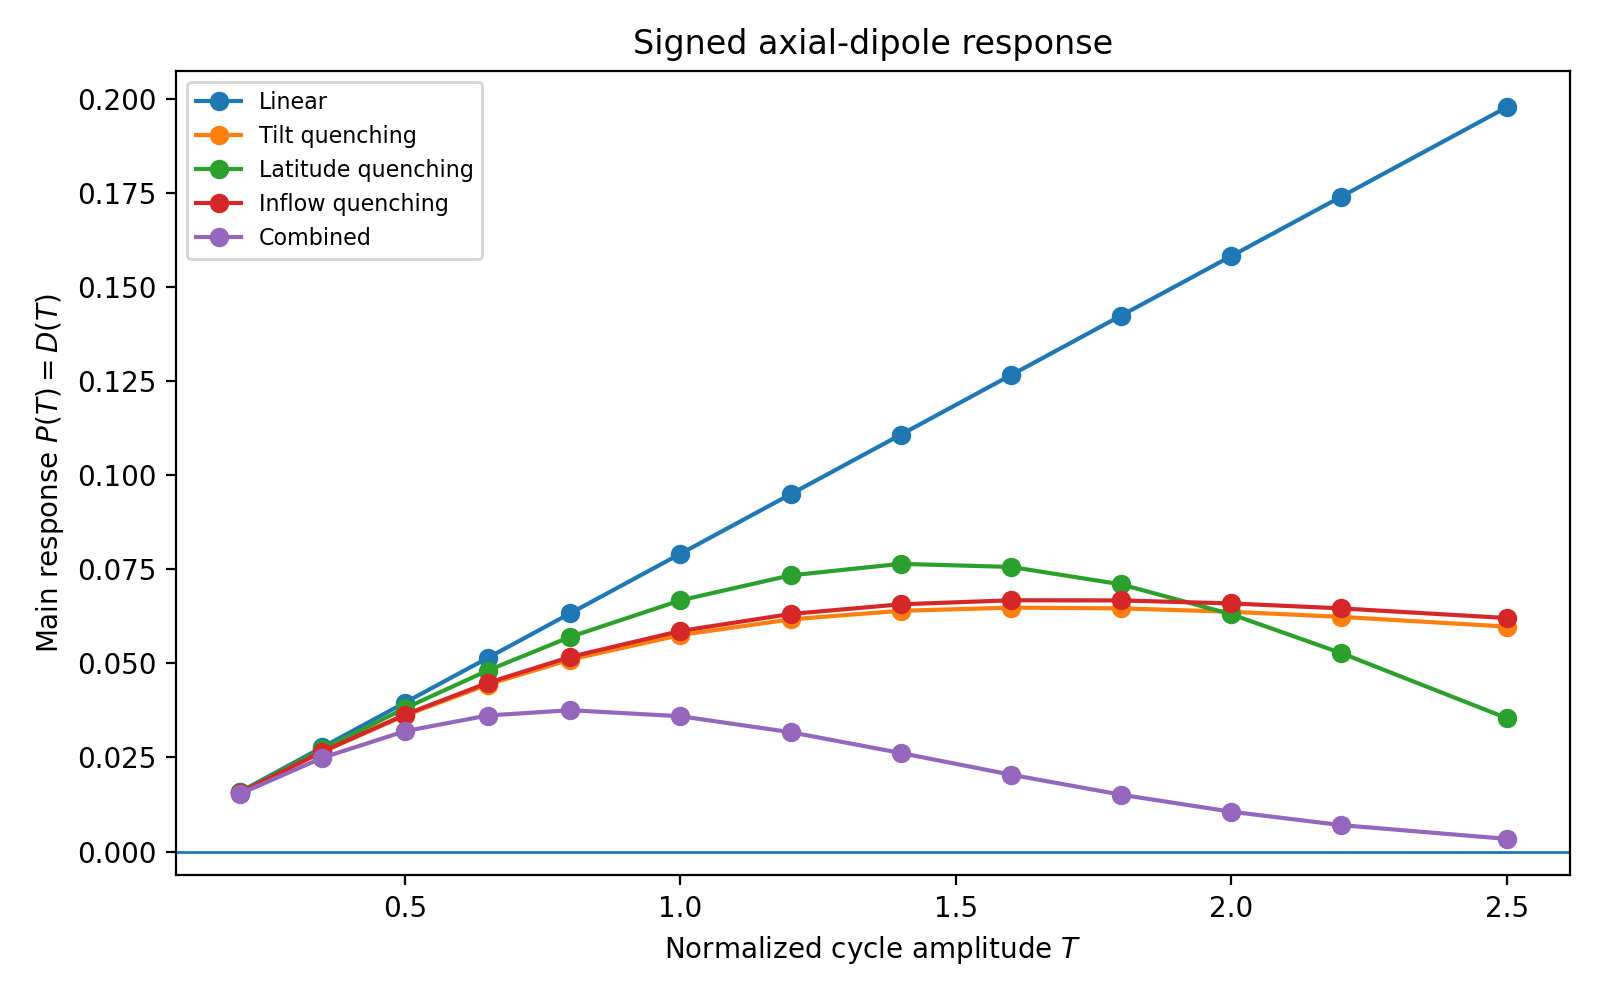
\includegraphics[width=\linewidth]{fig1_main_signed_axial_dipole_response_raw.png}
\caption{Signed axial-dipole response $P(T)=D(T)$ as a function of
normalised cycle amplitude. This is the main raw SFT diagnostic used in
the reduced response analysis.}
\label{fig:signed_dipole}
\end{figure}

\begin{figure}
\centering
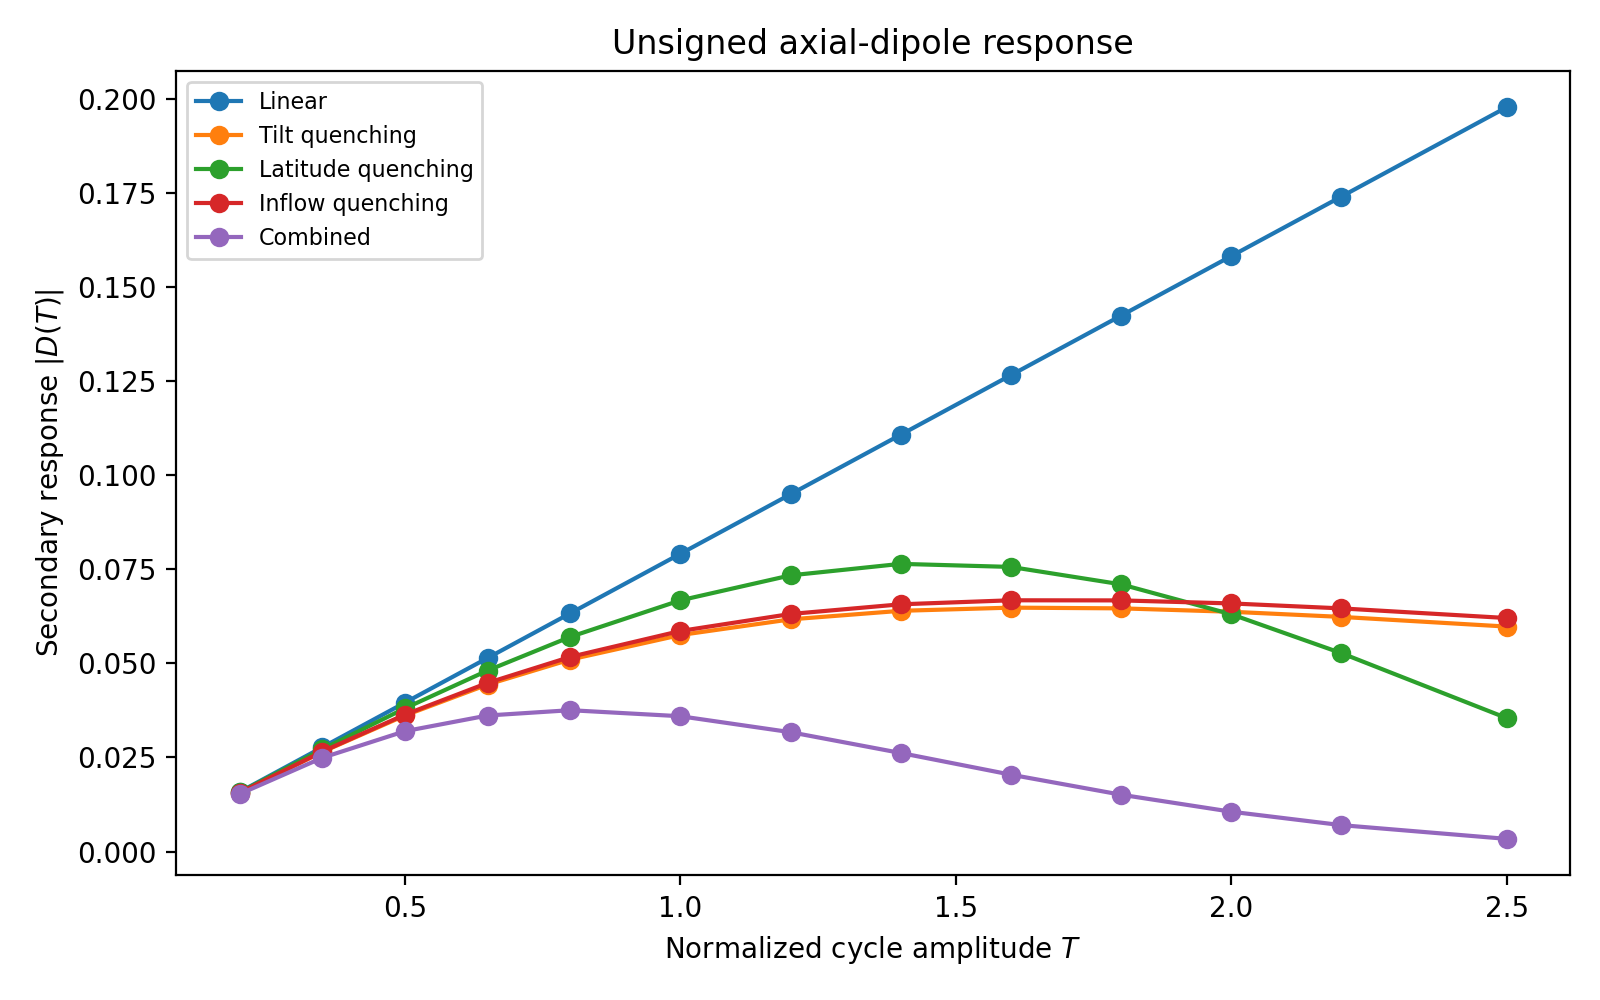
\includegraphics[width=\linewidth]{fig1b_unsigned_axial_dipole_response.png}
\caption{Unsigned axial-dipole response $|D(T)|$ as a function of
normalised cycle amplitude $T$. The nonlinear cases show saturation and
suppression relative to the linear reference case.}
\label{fig:unsigned_dipole}
\end{figure}

\subsection{Normalised response compared with the reduced theory}

Figure~\ref{fig:normalized_response} is the central validation figure of
the controlled experiments: the normalised SFT response
$\hat{P}(T)=P(T)/P(1)$ against the reduced prediction $TQ(T)/Q(1)$. The
quantitative agreement is summarised in
Table~\ref{tab:agreement}. The linear and inflow cases agree to round-off,
as linearity demands -- their agreement validates the code rather than the
theory. The tilt case agrees to $2.0$~per~cent (the geometric
linearisation of Section~\ref{subsec:tilt_quenching_equation}), and the
latitude case to $7.0$~per~cent at the extreme of the scan (the
envelope-average closure of Section~\ref{subsec:lq_equation}; below
$2$~per~cent for $T\le1.2$). The combined case is more accurate in
absolute terms than the latitude case because the tilt and latitude
residuals partially cancel.

\begin{table}
\caption{Agreement between the normalised SFT response and the reduced
prediction over the scan $T\in[0.2,2.5]$.}
\label{tab:agreement}
\begin{tabular}{lcc}
\hline
Case & $\Delta_{\rm abs}^{\rm max}$ & $\Delta_{\rm rel}^{\rm max}$ \\
\hline
linear   & $<10^{-14}$ & $<10^{-14}$ \\
tilt     & $0.030$ & $2.0\%$ \\
latitude & $0.066$ & $7.0\%$ \\
inflow   & $<10^{-14}$ & $<10^{-14}$ \\
combined & $0.016$ & $5.0\%$ \\
\hline
\end{tabular}
\end{table}

\begin{figure}
\centering
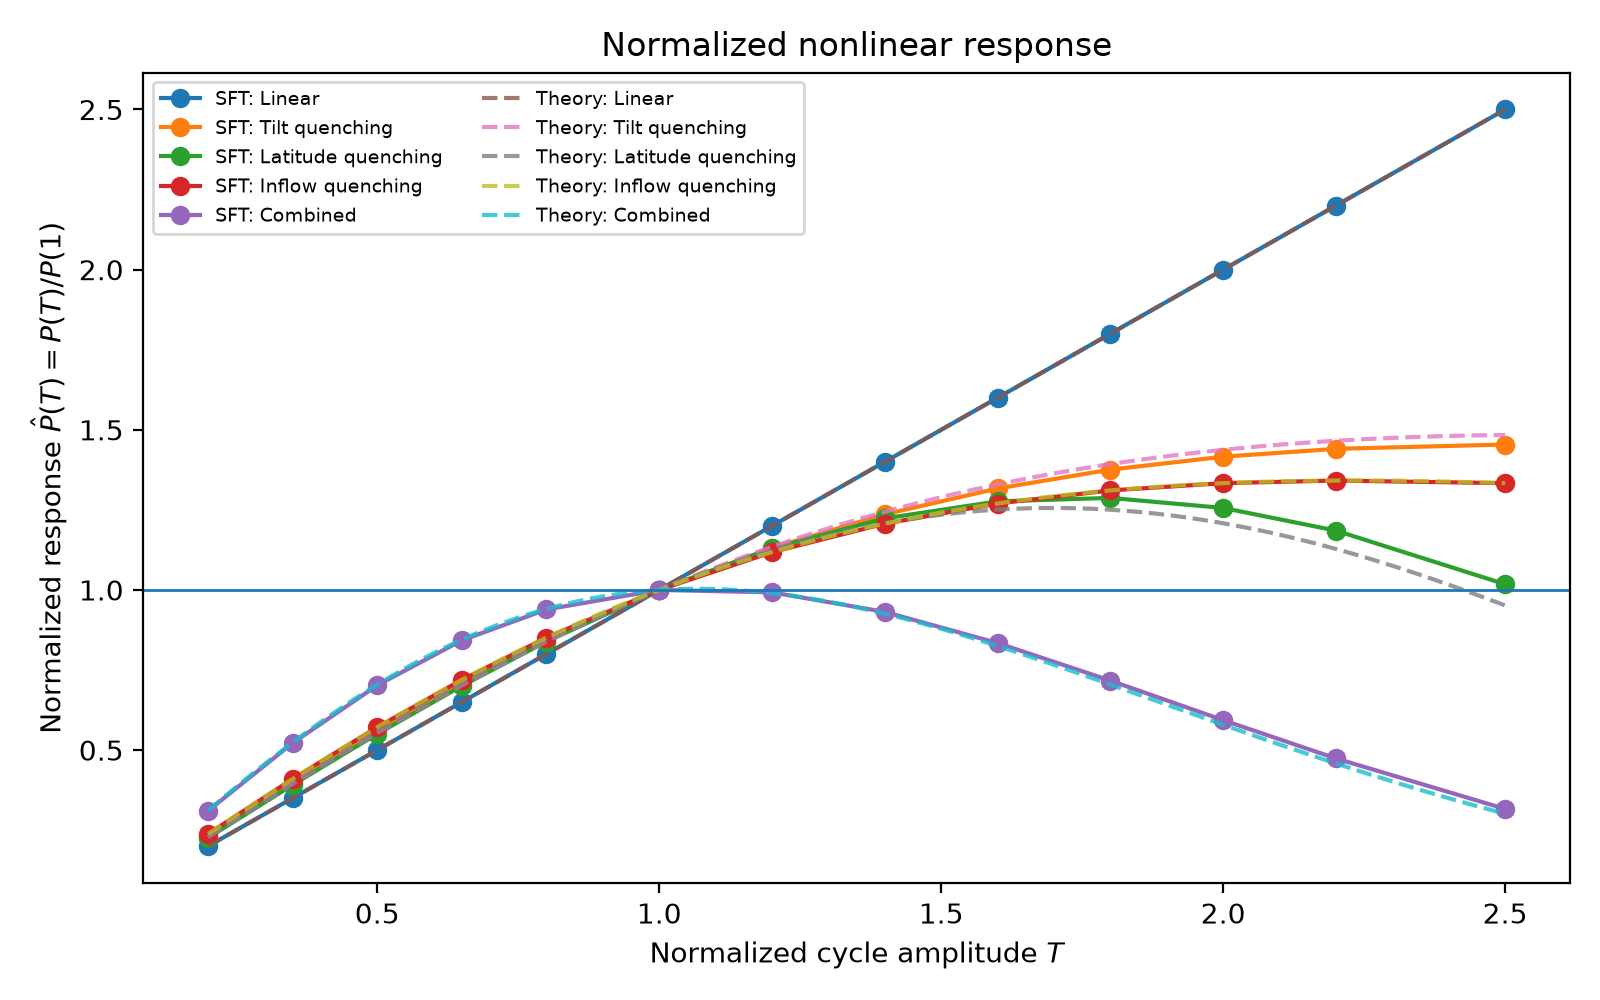
\includegraphics[width=\linewidth]{fig2_normalized_response_vs_theory.png}
\caption{Normalised nonlinear response $\hat{P}(T)=P(T)/P(1)$ compared
with the reduced-theory prediction $TQ(T)/Q(1)$. The agreement confirms
the consistency of the reduced response formulation in the controlled SFT
set-up; the quantitative deviations are listed in
Table~\ref{tab:agreement}.}
\label{fig:normalized_response}
\end{figure}

\subsection{Nonlinear response function}

Figure~\ref{fig:response_function} shows the normalised nonlinear response
function $\mathcal{R}(T)=\rmd\hat{P}/\rmd T$. For the linear case
$\mathcal{R}\simeq1$; in the tilt-like and inflow-like cases the response
decreases gradually towards zero (saturation); in the latitude-like case
it becomes negative at large amplitudes; and the combined case becomes
negative earliest and most strongly. Through the identity
(\ref{eq:R_M_identity}), the measured response function directly locates
the cycle map relative to the onset of modulation.

\begin{figure}
\centering
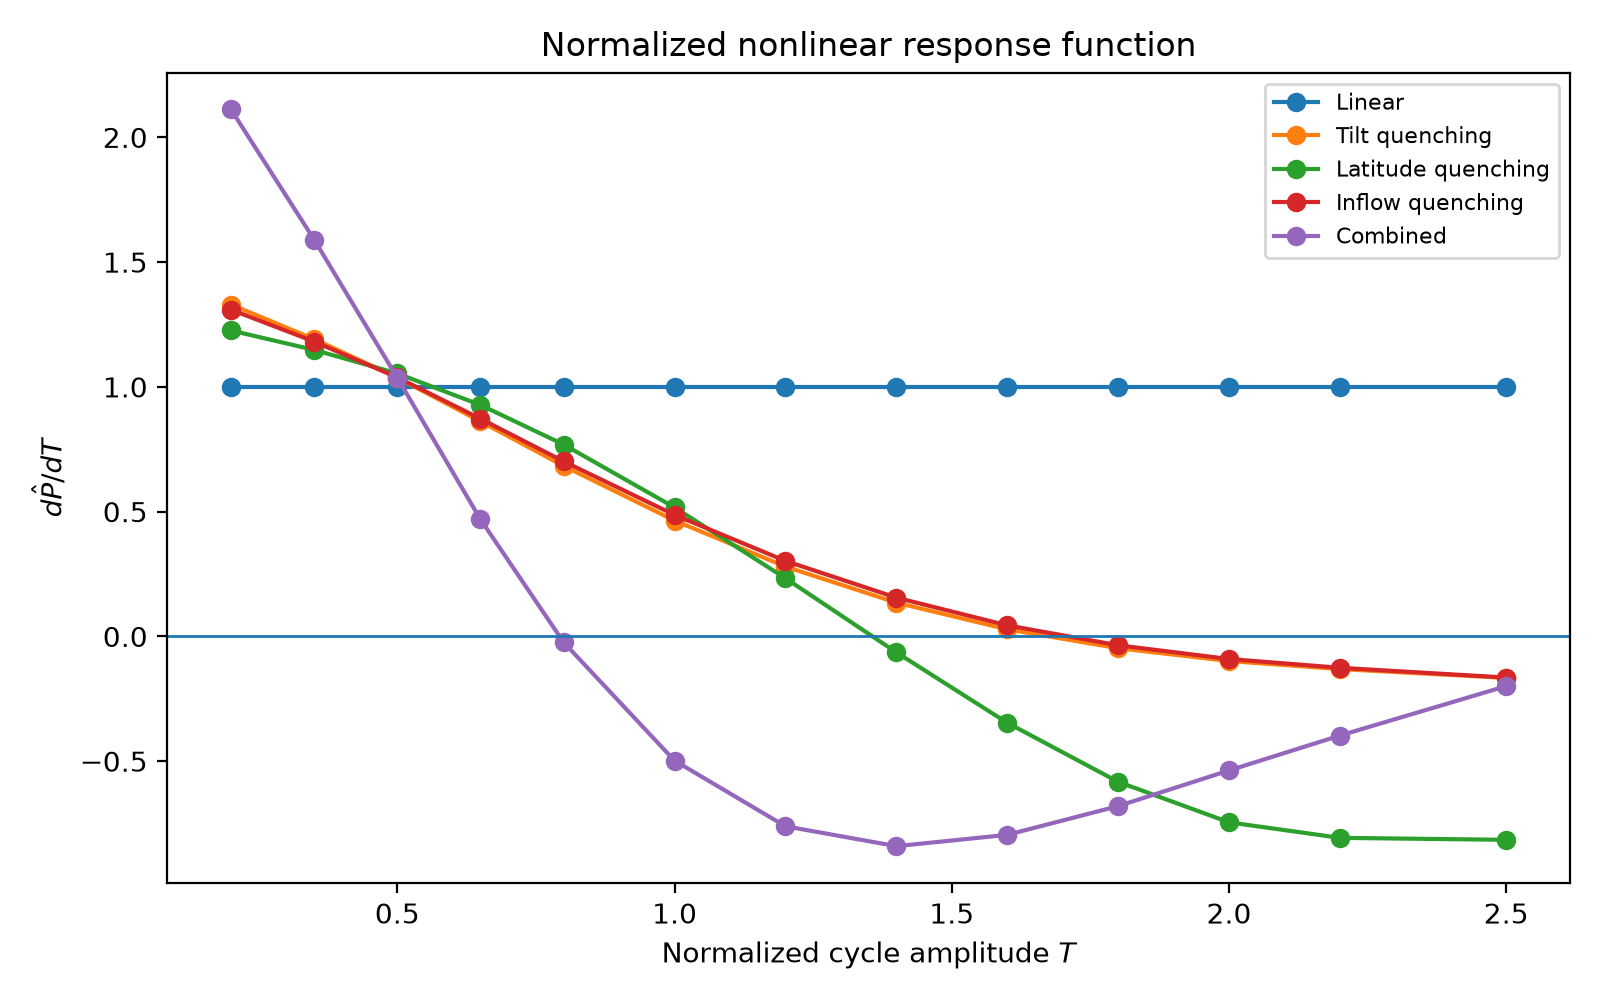
\includegraphics[width=\linewidth]{fig3_normalized_nonlinear_response.png}
\caption{Normalised nonlinear response function $\rmd\hat{P}/\rmd T$.
Positive values indicate normal dipole build-up, values near zero indicate
saturation, and negative values indicate an over-quenched response.}
\label{fig:response_function}
\end{figure}

\subsection{Polar-cap field response}

Figure~\ref{fig:polar_cap} shows the polar-cap proxy as a secondary
diagnostic. The qualitative trends follow the axial-dipole response, but
the proxy depends on the chosen polar-cap threshold; the signed axial
dipole, being a global integral directly connected to the poloidal field,
remains the main diagnostic.

\begin{figure}
\centering
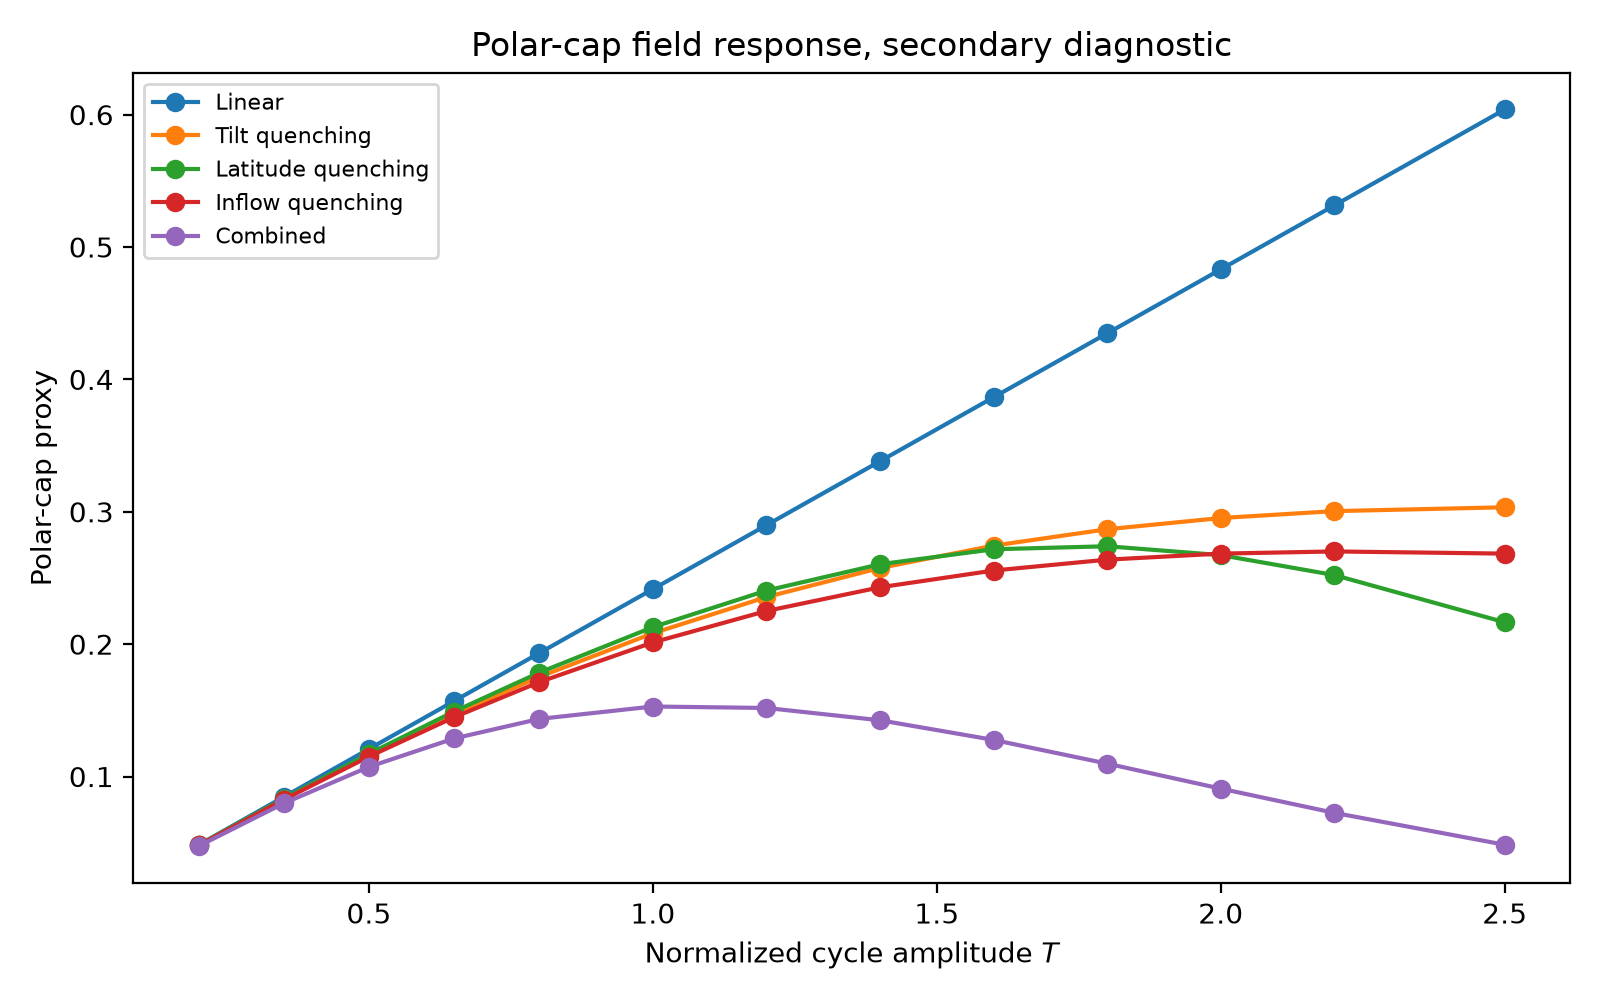
\includegraphics[width=\linewidth]{fig5_polar_cap_response_secondary.png}
\caption{Polar-cap field proxy as a secondary diagnostic. The qualitative
trends are consistent with the axial-dipole response.}
\label{fig:polar_cap}
\end{figure}

\subsection{Reduced nonlinear efficiency factors and effective gain}

Figure~\ref{fig:q_efficiency} shows the efficiency factors themselves. The
tilt-like and inflow-like factors decrease algebraically,
Equations~(\ref{eq:QTQ}) and~(\ref{eq:QI}); the belt-consistent
latitude-like factor, Equation~(\ref{eq:QLQ_belt}), decreases more rapidly
because of its exponential dependence; and the combined factor declines
fastest. Figure~\ref{fig:effective_gain} translates this into the
effective gain $D_{\rm eff}(T)=D_0Q(T)$ for the illustrative value
$D_0=3$ (the same gain as the stability maps below): finite-amplitude
saturation occurs where $D_{\rm eff}=1$, which the combined case reaches
at the lowest amplitude.

\begin{figure}
\centering
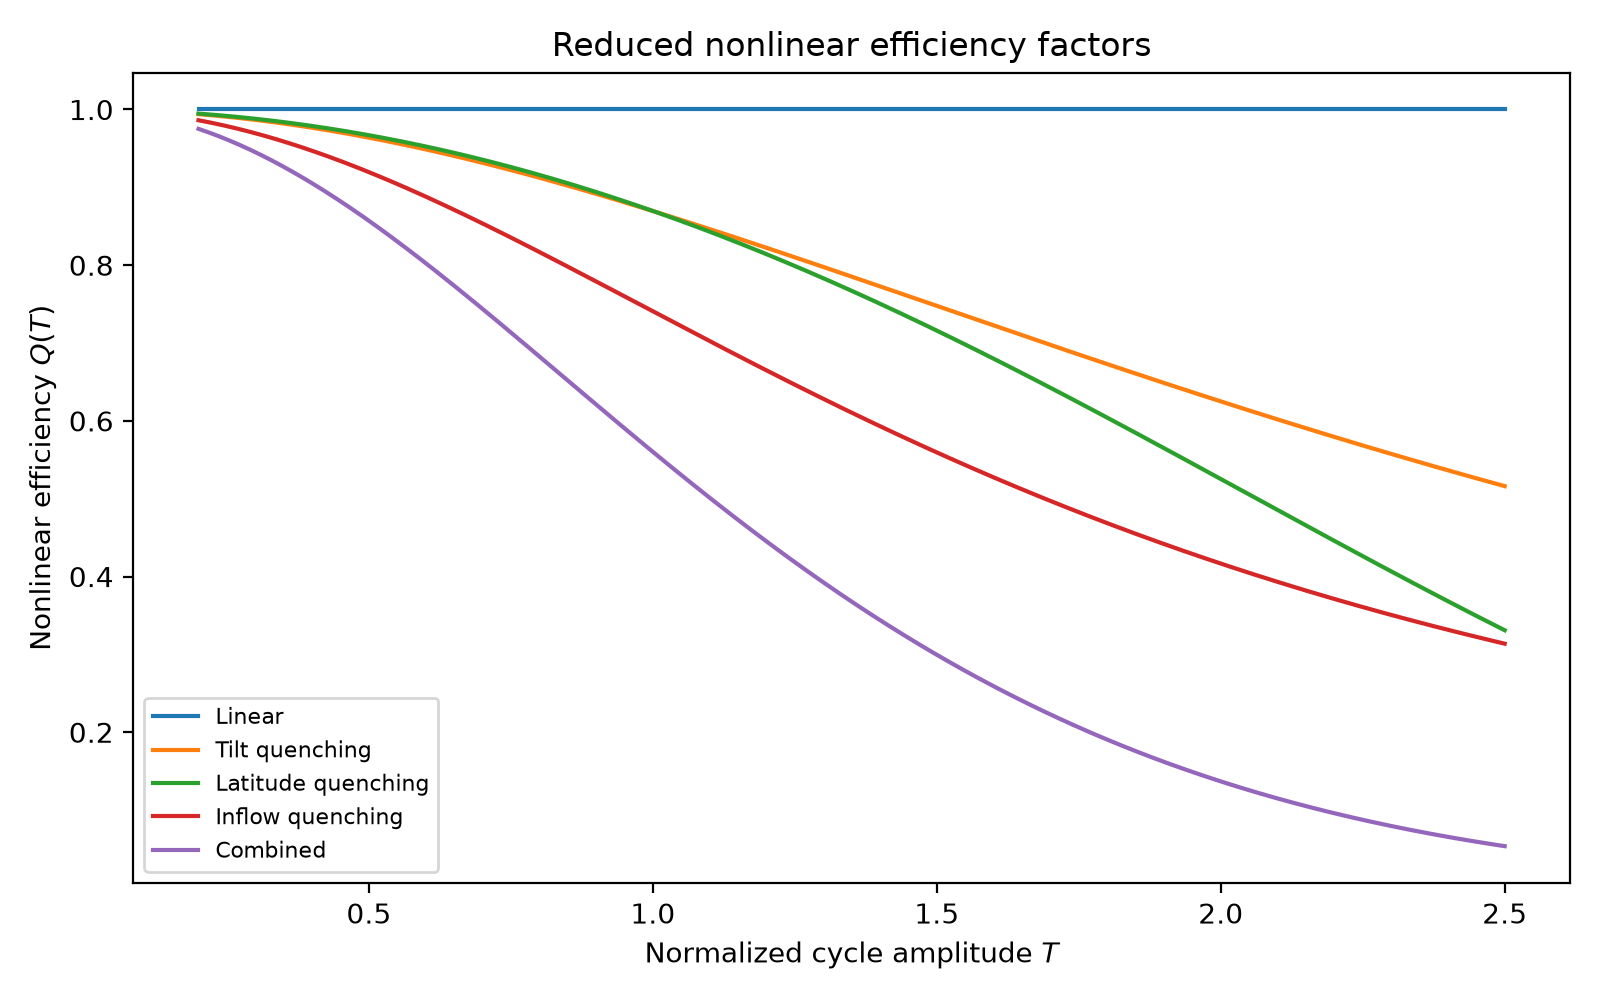
\includegraphics[width=\linewidth]{fig6_Q_efficiency.png}
\caption{Reduced nonlinear efficiency factors $Q(T)$ used in the
controlled experiments. The combined factor decreases fastest because the
individual factors multiply.}
\label{fig:q_efficiency}
\end{figure}

\begin{figure}
\centering
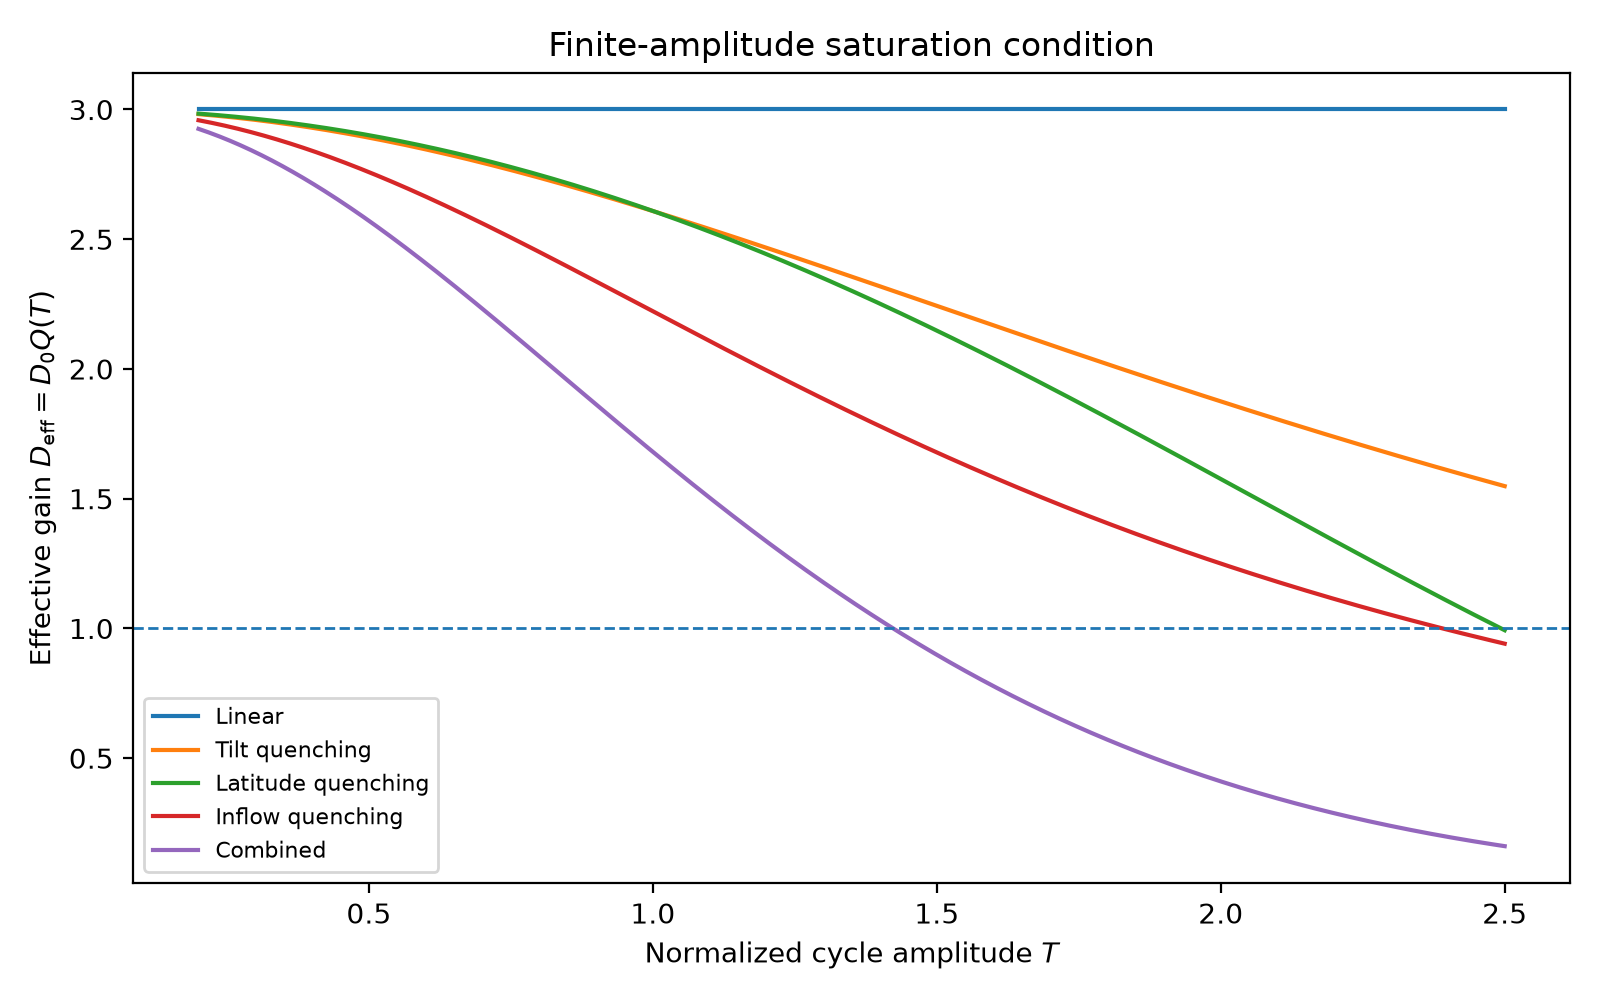
\includegraphics[width=\linewidth]{fig7_effective_gain.png}
\caption{Finite-amplitude saturation condition in the reduced cycle map.
The effective gain is $D_{\rm eff}=D_0Q(T)$ with the illustrative gain
$D_0=3$, and saturation occurs where $D_{\rm eff}=1$.}
\label{fig:effective_gain}
\end{figure}

\subsection{Final latitude profiles for the combined case}

Figure~\ref{fig:final_profiles} shows the final surface field profiles for
selected amplitudes in the combined case: for small and moderate
amplitudes the polar fields strengthen with $T$, while at $T=2.5$ the
combined efficiency factor strongly suppresses the source and the final
field is much weaker.

\begin{figure}
\centering
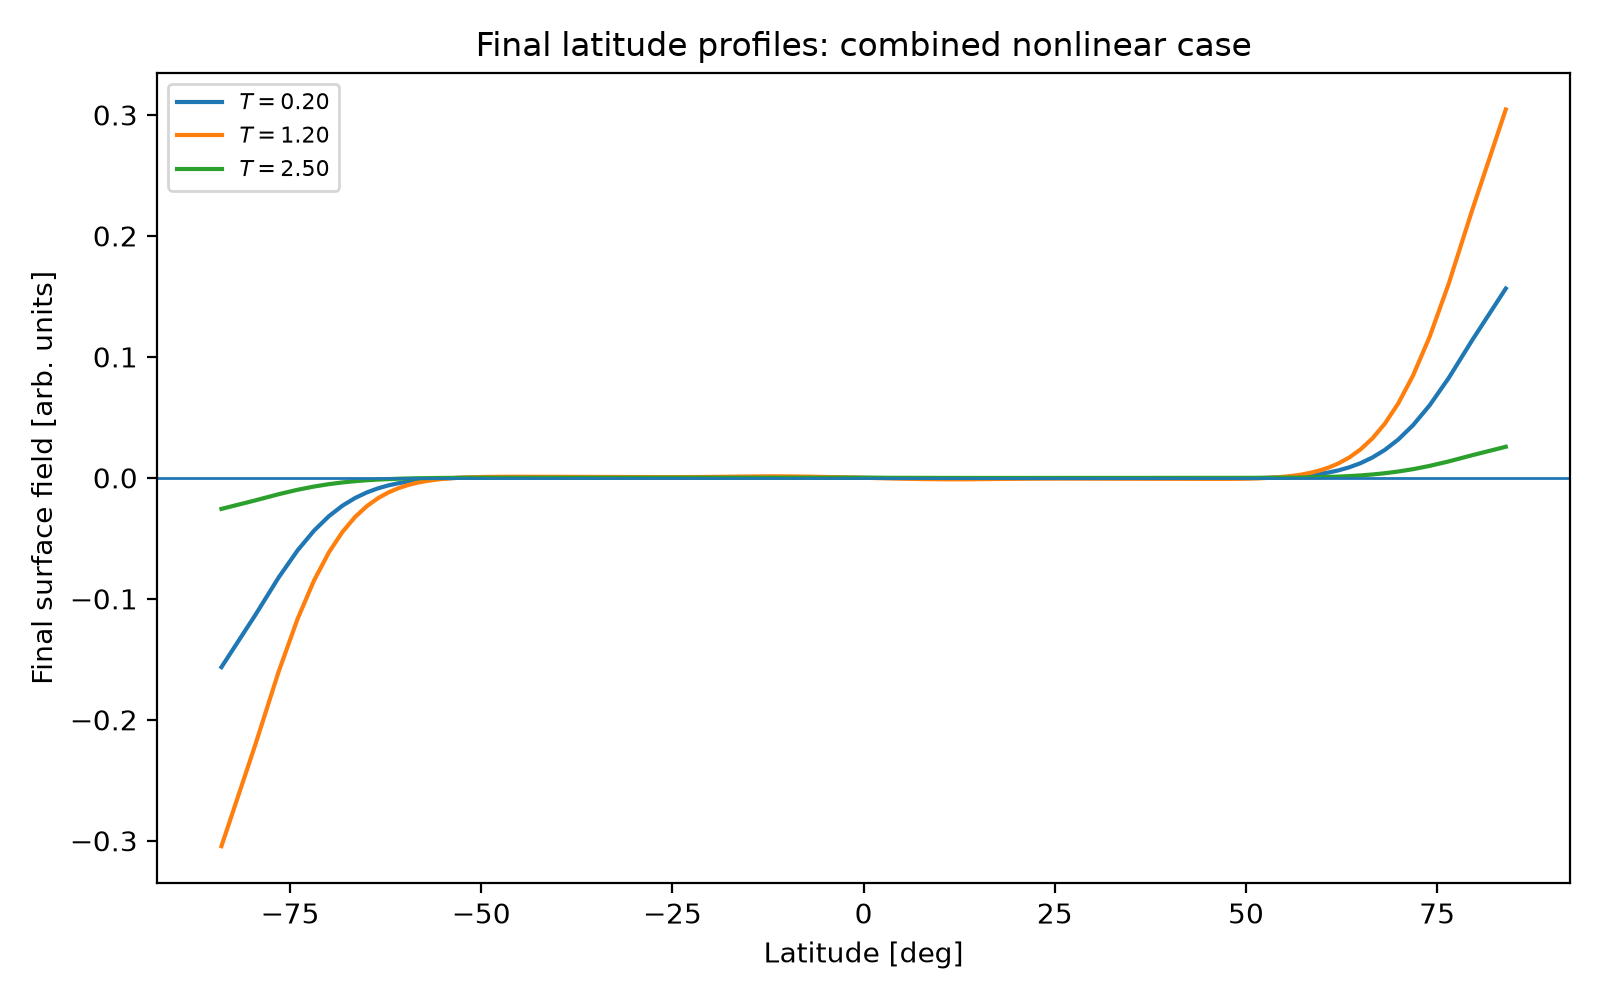
\includegraphics[width=\linewidth]{fig8_final_profiles_combined.png}
\caption{Final latitude profiles of the surface field for selected
amplitudes in the combined nonlinear case.}
\label{fig:final_profiles}
\end{figure}

\subsection{Stability maps of the reduced cycle map}

Figures~\ref{fig:stability_map}\,--\,\ref{fig:mprime_map} classify the
reduced cycle map in the $(b_{\rm TQ},b_{\rm LQ})$ plane at $D_0=3$: the
stability classification with the analytic period-doubling boundary
$\mathcal{M}'(T_*)=-1$ overlaid, the saturated amplitude $T_*$, and the
multiplier $\mathcal{M}'(T_*)$. The structure follows the analytic results
of Section~\ref{subsec:cycle_map_stability}: instability is entered far
more readily by increasing the Gaussian latitude-quenching strength, whose
stiffness is unbounded, than the algebraic tilt-quenching strength, which
can never destabilise the map on its own; increasing $b_{\rm TQ}$ at fixed
gain in fact lowers $T_*$ and thereby stabilises the map.

\begin{figure}
\centering
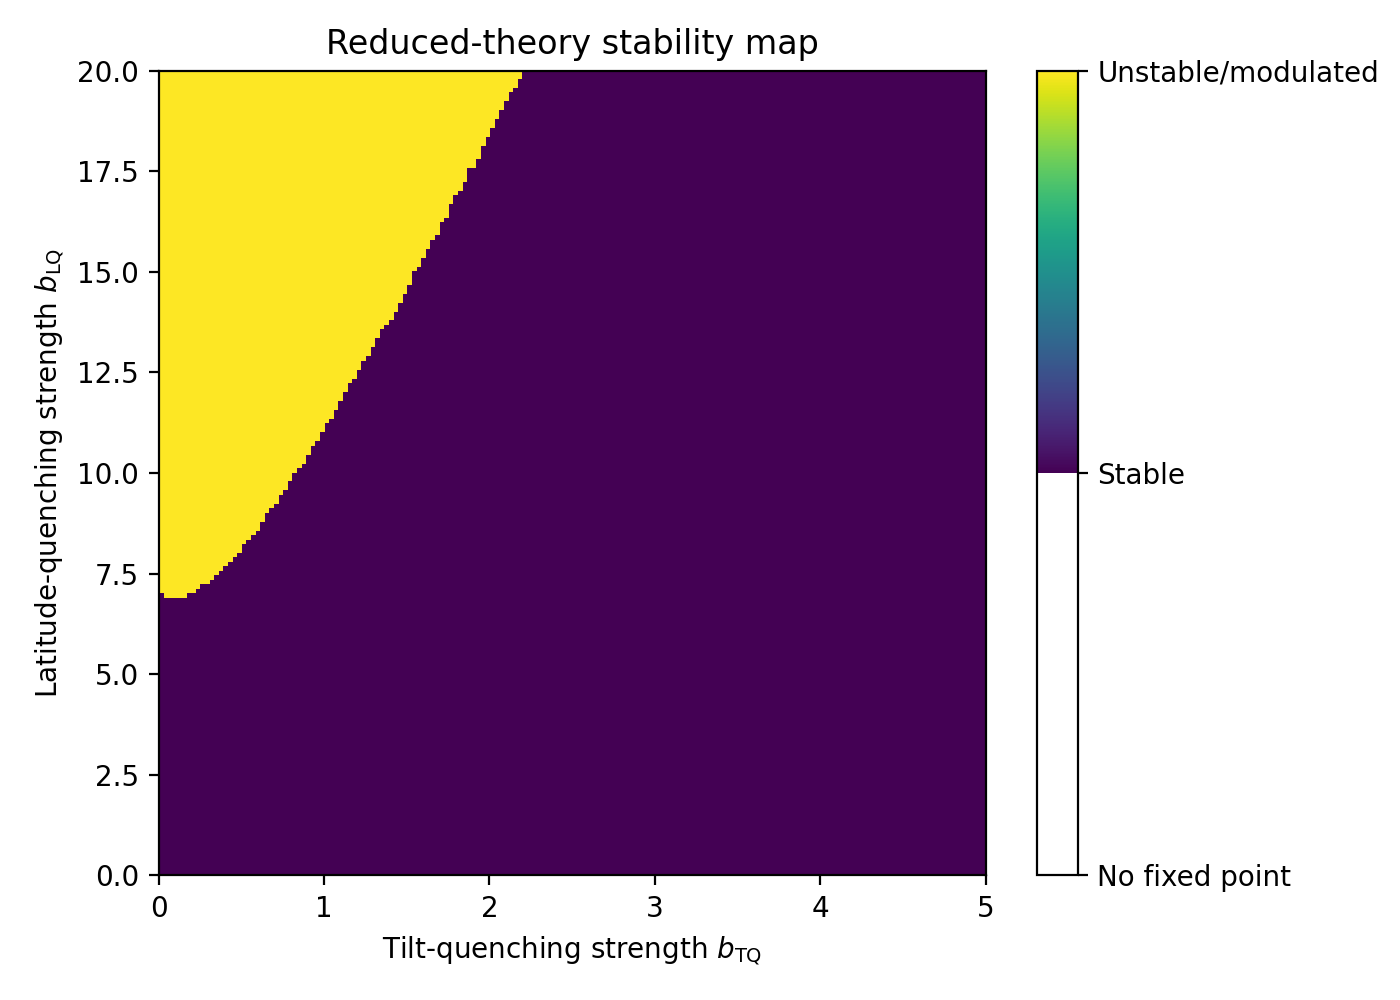
\includegraphics[width=0.85\linewidth]{fig9_stability_map_classification.png}
\caption{Reduced-theory stability map for the cycle map
$T_{n+1}=D_0T_nQ(T_n)$. Stable regions satisfy $|\mathcal{M}'(T_*)|<1$;
the dashed curve is the analytic period-doubling boundary
$\mathcal{M}'(T_*)=-1$.}
\label{fig:stability_map}
\end{figure}

\begin{figure}
\centering
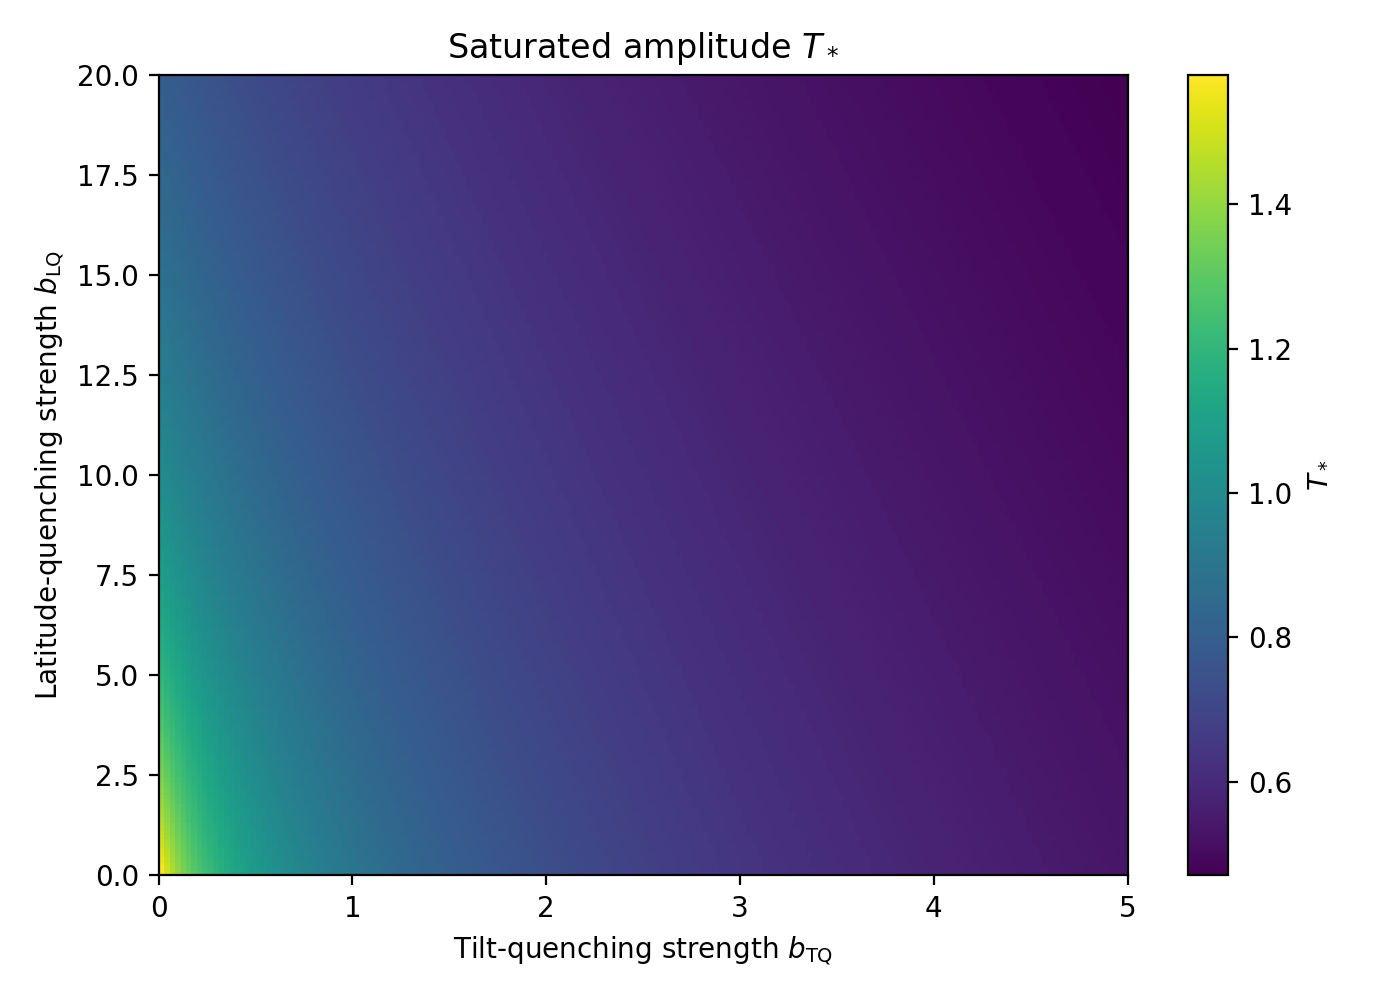
\includegraphics[width=0.85\linewidth]{fig10_Tstar_map.png}
\caption{Saturated amplitude $T_*$ from the fixed-point condition
$D_0Q(T_*)=1$. Stronger nonlinear feedbacks reduce the equilibrium
amplitude.}
\label{fig:tstar_map}
\end{figure}

\begin{figure}
\centering
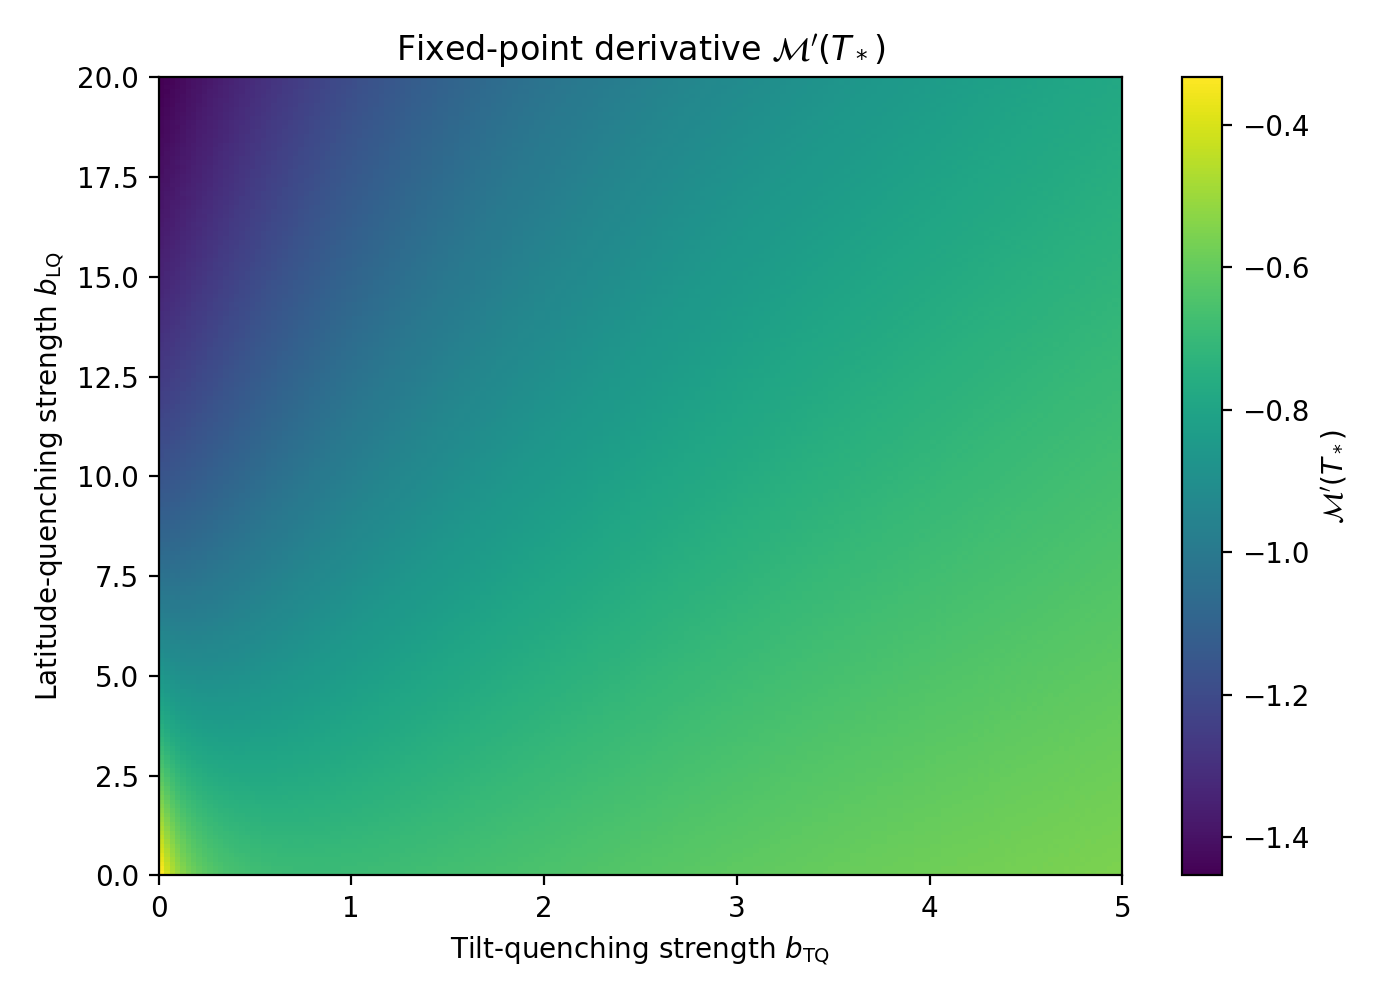
\includegraphics[width=0.85\linewidth]{fig11_Mprime_map.png}
\caption{Fixed-point multiplier $\mathcal{M}'(T_*)$ of the reduced cycle
map. Stable fixed points satisfy $-1<\mathcal{M}'(T_*)<1$.}
\label{fig:mprime_map}
\end{figure}

\section{The Adjoint-Kernel Framework}
\label{sec:kernel_framework}

The reduction $P=aTQ(T)$ is placed on an exact footing by making the
kernel of Equation~(\ref{eq:kernel_identity}) explicit at the discrete
level. Writing the solver's update as
$B^{k+1}=\Pi M^{-1}[(I+\Delta t\,\mathsf{A})B^{k}+\Delta t\,S^{k}]$, with
$\mathsf{A}$ the explicit (advection $+$ decay) operator, $M$ the
symmetric implicit-diffusion matrix, and $\Pi$ the monopole projection,
the final dipole $D=w^{\rm T}B^{N}$ becomes exactly
%
\begin{equation}
D=\sum_{k}\omega_k,
\qquad
\omega_k=\Delta t\,(K^{k})^{\rm T}S^{k},
\label{eq:discrete_duality}
\end{equation}
%
with the kernel obtained by one backward recursion,
$K^{N-1}=M^{-1}\Pi w$ and
$K^{k-1}=M^{-1}\Pi(I+\Delta t\,\mathsf{A})^{\rm T}K^{k}$. Numerically, the
adjoint sum and the forward linear run agree to a relative difference of
$1.9\times10^{-15}$, recovering $a=7.899\times10^{-2}$. One adjoint solve
therefore replaces the entire amplitude scan for \emph{any} source-side
nonlinearity: by linearity, $D(T)=T\sum_k\omega_k\,Q_X(t_k,T)$ exactly.

\subsection{Closure ladder for latitude quenching}
\label{subsec:closure_ladder}

Truncating the cumulant expansion of this exact kernel-weighted average
produces a ladder of closures for the latitude case, each evaluated
against the stored SFT scan (Figure~\ref{fig:closure_ladder} and
Table~\ref{tab:ladder}). The default envelope closure's entire residual is
the covariance between the instantaneous quenching factor and the
time-dependence of the dipole yield: the true weighting $\omega(t)$ peaks
at $\bar{t}_\omega=6.5$~yr, two years \emph{after} cycle maximum, because
early-cycle flux emerges at high latitudes where its yield is small.
Replacing the envelope moments $(t_{\rm max},\sigma_t)$ in
Equations~(\ref{eq:lq_lambda_eff})\,--\,(\ref{eq:lq_epsilon}) by the
yield-weighted moments $(\bar{t}_\omega,\sigma_\omega)=(6.52,1.48)$~yr --
measurable from a single adjoint solve -- reduces the closure error by
three orders of magnitude while keeping the same closed form.

\begin{table}
\caption{Closure ladder for the latitude-quenching case: maximum absolute
deviation of the normalised response from the SFT scan.}
\label{tab:ladder}
\begin{tabular}{llc}
\hline
Closure level & Time weighting & $\Delta_{\rm abs}^{\rm max}$ \\
\hline
exact kernel average & $\omega_k$ (kernel $\times$ source) & $4\times10^{-11}$\,$^{\rm a}$ \\
yield-weighted Gaussian & $\bar{t}_\omega=6.52$~yr, $\sigma_\omega=1.48$~yr & $5.5\times10^{-5}$ \\
envelope Gaussian (default) & $t_{\rm max}=4.5$~yr, $\sigma_t=2.2$~yr & $6.6\times10^{-2}$ \\
static (fixed base latitude) & $\delta$-function at cycle end & $1.7\times10^{-1}$ \\
\hline
\end{tabular}\\
$^{\rm a}$ limited by the precision of the stored scan, not by the
identity.
\end{table}

\begin{figure}
\centering
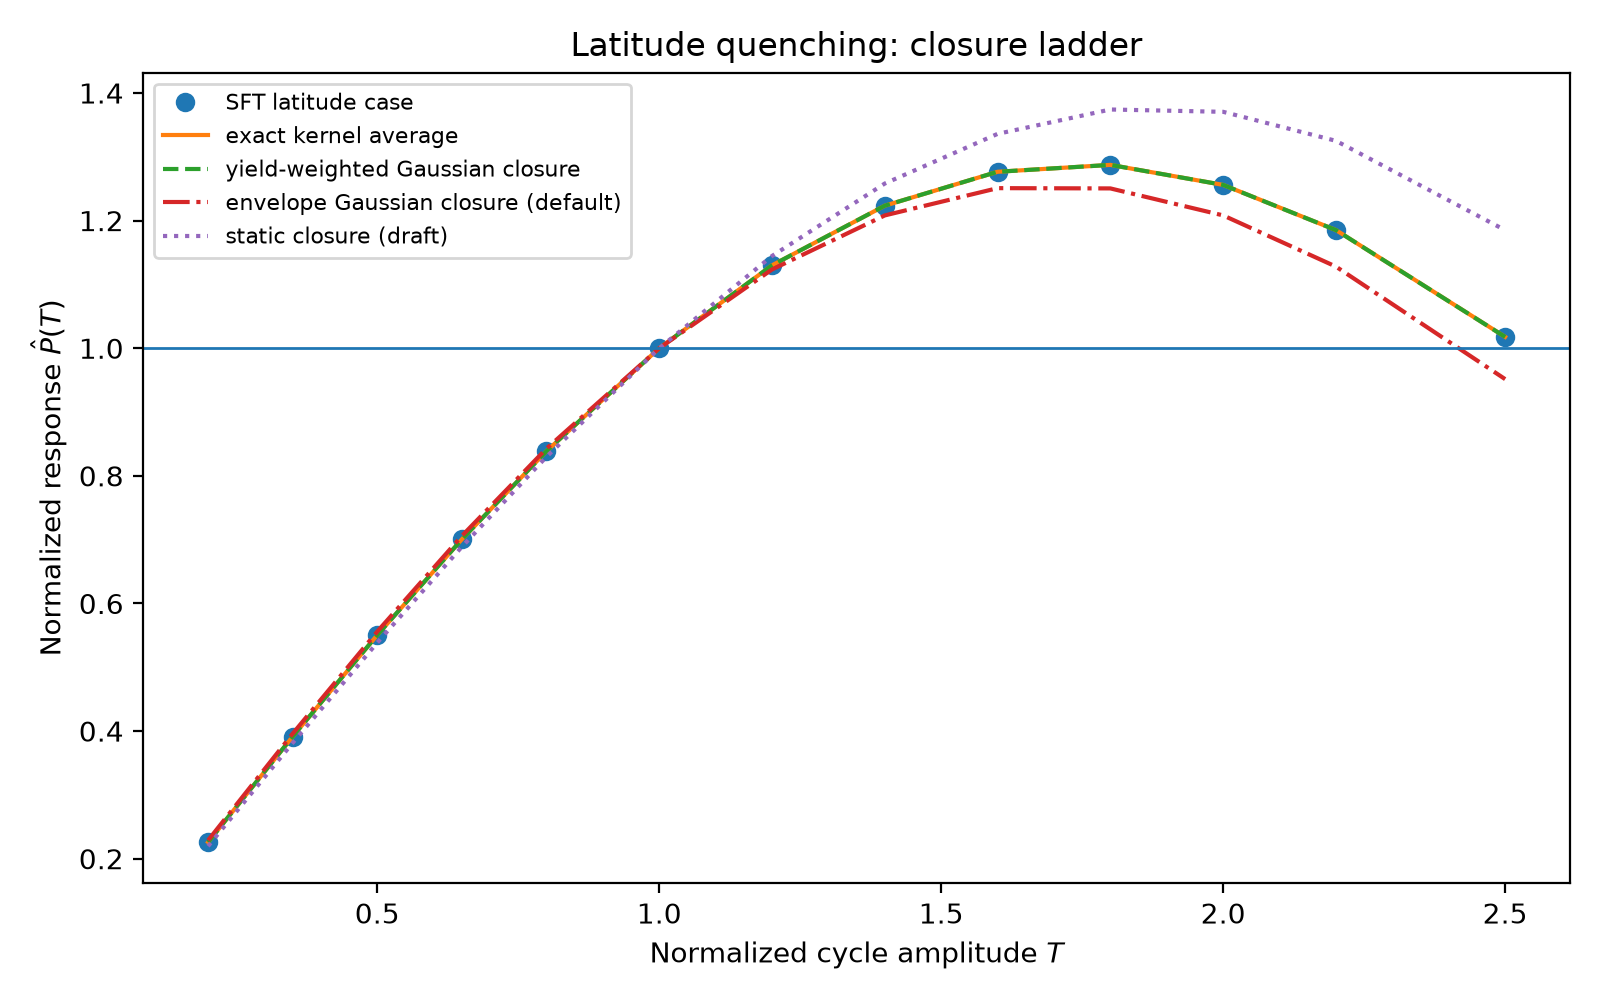
\includegraphics[width=\linewidth]{figF4_closure_ladder.png}
\caption{Closure ladder for latitude quenching: the SFT scan, the exact
kernel average, the yield-weighted Gaussian closure, the default envelope
closure, and the static closure of the earlier formulation.}
\label{fig:closure_ladder}
\end{figure}

\subsection{Effectivity ranges of the transport model}
\label{subsec:effectivity_ranges}

The kernel also measures the dynamo effectivity range of the transport
model directly. The yield of a point source at latitude $\lambda$,
relative to the dipole it deposits, is approximately Gaussian with width
$29.2^\circ$ at the reference parameters (converged already within the
11-yr window). The physically relevant quantity for bipolar regions,
however, is the yield of the \emph{ring pair}, which is much narrower --
$\lambda_R^{\rm pair}=10.5^\circ$ -- and changes sign at
$\lambda_{\rm rev}\approx25^\circ$: pairs emerging poleward of this
latitude contribute to the final dipole with reversed sign. The prescribed
closure parameter $\lambda_R=20^\circ$ in
Equation~(\ref{eq:nonlinear_reference_params}) is therefore a free
demonstration value rather than the model's own; the consequences of the
distinction appear in Section~\ref{sec:physical_validation}, and the
scaling of $\lambda_R^{\rm pair}$ with the transport parameters is
established in Section~\ref{sec:parameter_space}.

\section{Physical Validation of the Closures}
\label{sec:physical_validation}

The controlled experiments prescribe the efficiency factors; this section
confronts the theory with the \emph{physical} implementations of the
nonlinearities, using only kernel-derived quantities.

\subsection{Tilt quenching: exact prediction and improved closure}

The tilt case changes the source geometry, so it is not a scalar source
factor; nevertheless the kernel predicts the scan exactly (maximum
relative error $1\times10^{-14}$; Figure~\ref{fig:tilt_exact}), because
the response to any source is available once the kernel is known. The
cycle-aggregated yield as a function of polarity separation is measured to
be $A(s)=c_1s+c_3s^3$ with $c_3/c_1=+1.7\times10^{-3}~{\rm deg}^{-2}$,
confirming the odd-yield structure asserted in
Section~\ref{subsec:tilt_quenching_equation}. The improved closure
%
\begin{equation}
Q_{\rm TQ}(T)
=
\frac{A(\Delta\lambda_0f_{\rm TQ}(T))}{A(\Delta\lambda_0)}
\label{eq:improved_tilt}
\end{equation}
%
reduces the closure error from $0.030$ to $1\times10^{-4}$; the naive
$Q_{\rm TQ}=f_{\rm TQ}$ remains a good approximation, its error now with a
measured, first-principles origin.

\begin{figure}
\centering
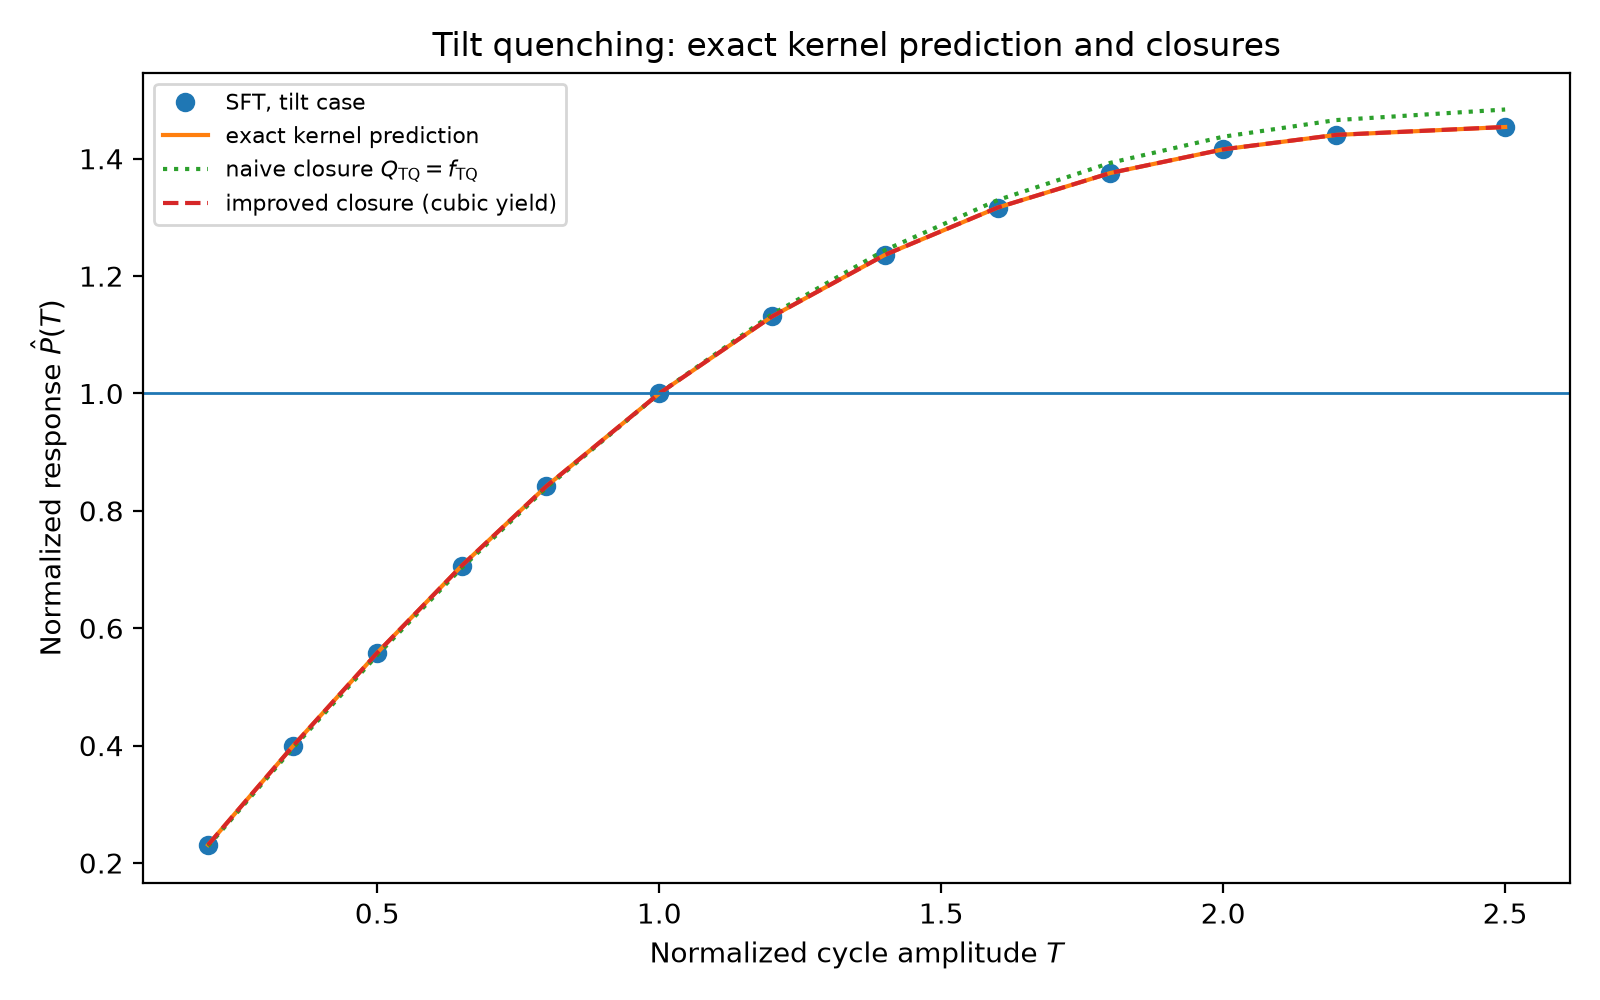
\includegraphics[width=\linewidth]{figV3_tilt_exact.png}
\caption{Tilt quenching: the SFT scan, the exact kernel prediction, the
naive closure $Q_{\rm TQ}=f_{\rm TQ}$, and the improved cubic-yield
closure of Equation~(\ref{eq:improved_tilt}).}
\label{fig:tilt_exact}
\end{figure}

\subsection{Physical latitude quenching and the sign reversal}

Figure~\ref{fig:pair_yield} shows the dipole yield of the ring-pair
structure versus its centre latitude, with the Gaussian fit
$\lambda_R^{\rm pair}=10.5^\circ$ and the sign change at
$\lambda_{\rm rev}\approx25^\circ$. When latitude quenching is implemented
physically -- the belt displaced poleward by
$\delta\lambda=b_{\rm LQ}T^2$ -- the response follows the kernel
prediction exactly (maximum relative error $2\times10^{-13}$) and
\emph{reverses sign} at $T_{\rm rev}=1.11$
(Figure~\ref{fig:shift_validation}): for stronger cycles the belt spends
enough of the cycle poleward of $\lambda_{\rm rev}$ that the
negative-yield contributions win. No positive multiplicative closure can
follow this: even with every ingredient derived (the pair effectivity
range and the yield-weighted moments), the Gaussian closure deviates by up
to $0.30$ in $Q$ already in the weak-shift domain $T\le0.8$, because near
the sign change the yield falls linearly through zero while any Gaussian
ratio falls log-linearly.

Two conclusions follow. First, efficiency-mode and shift-mode latitude
quenching with the same nominal $b_{\rm LQ}$ are \emph{not equivalent} in
this transport regime: matching even the weak-shift behaviour of the
physical displacement within the efficiency closure at $\lambda_R=20^\circ$
would require a strength about $(20/10.5)^2\approx3.6$ times larger.
Second, the reduced theory with positive $Q$ has a sharp domain boundary,
which Section~\ref{sec:parameter_space} expresses directly in transport
parameters.

\begin{figure}
\centering
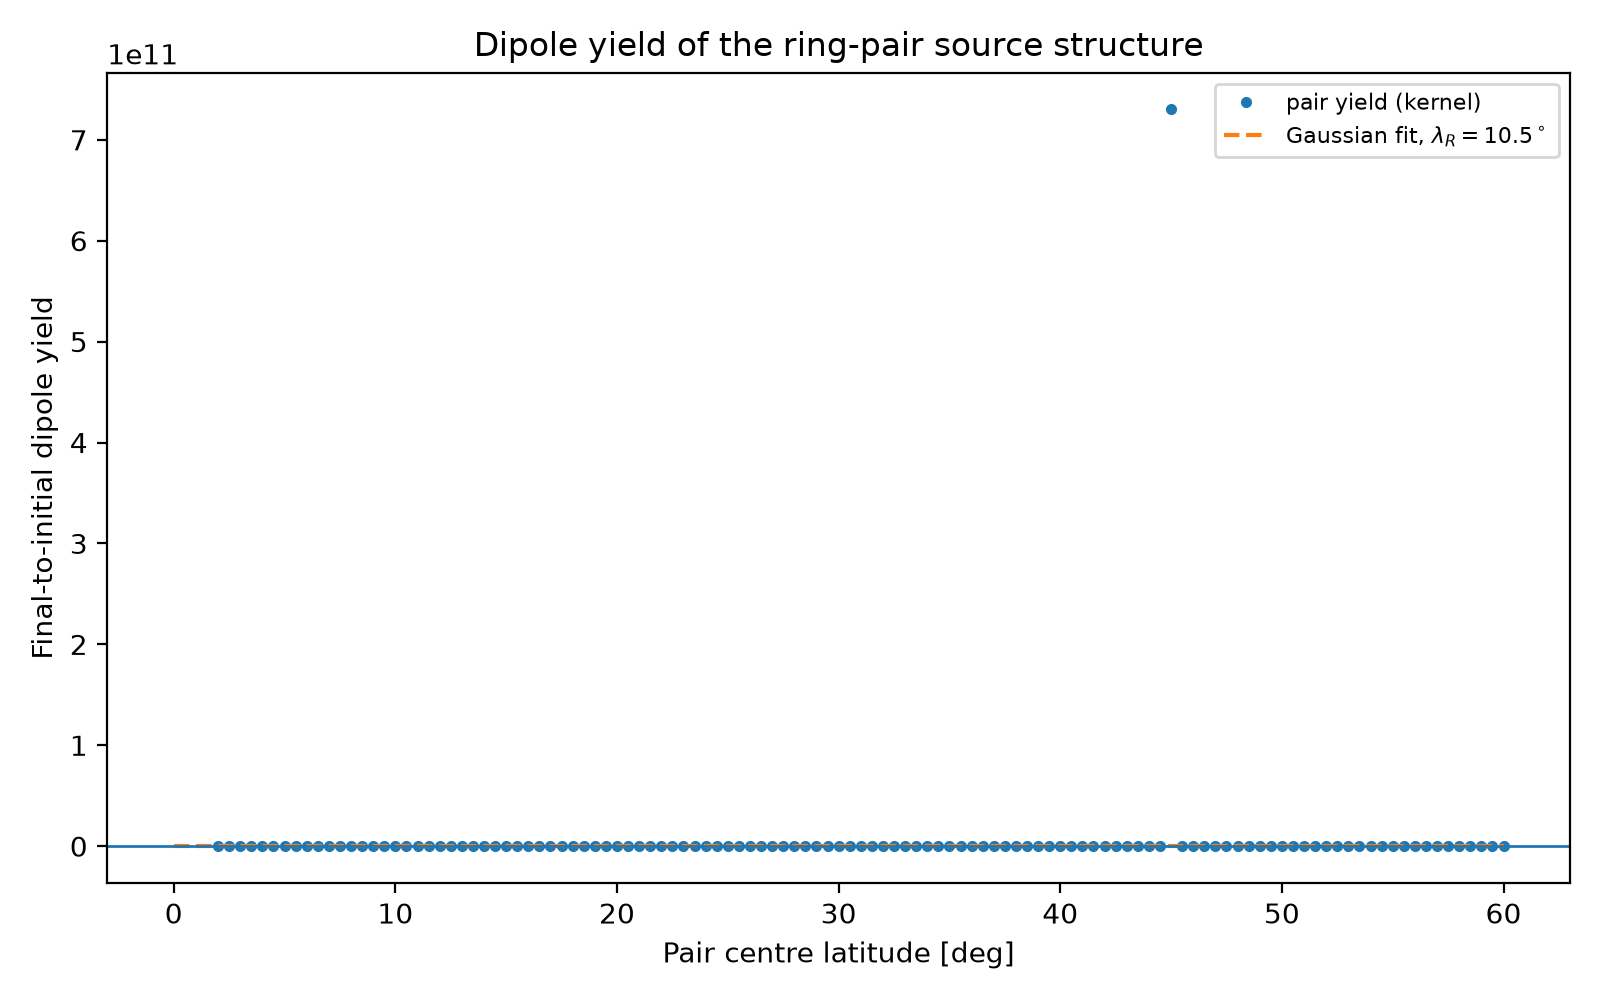
\includegraphics[width=\linewidth]{figV1_pair_yield.png}
\caption{Dipole yield of the ring-pair source structure versus its centre
latitude, from the asymptotic kernel. The Gaussian fit over the activity
belt gives $\lambda_R^{\rm pair}=10.5^\circ$; the yield changes sign at
$\lambda_{\rm rev}\approx25^\circ$.}
\label{fig:pair_yield}
\end{figure}

\begin{figure}
\centering
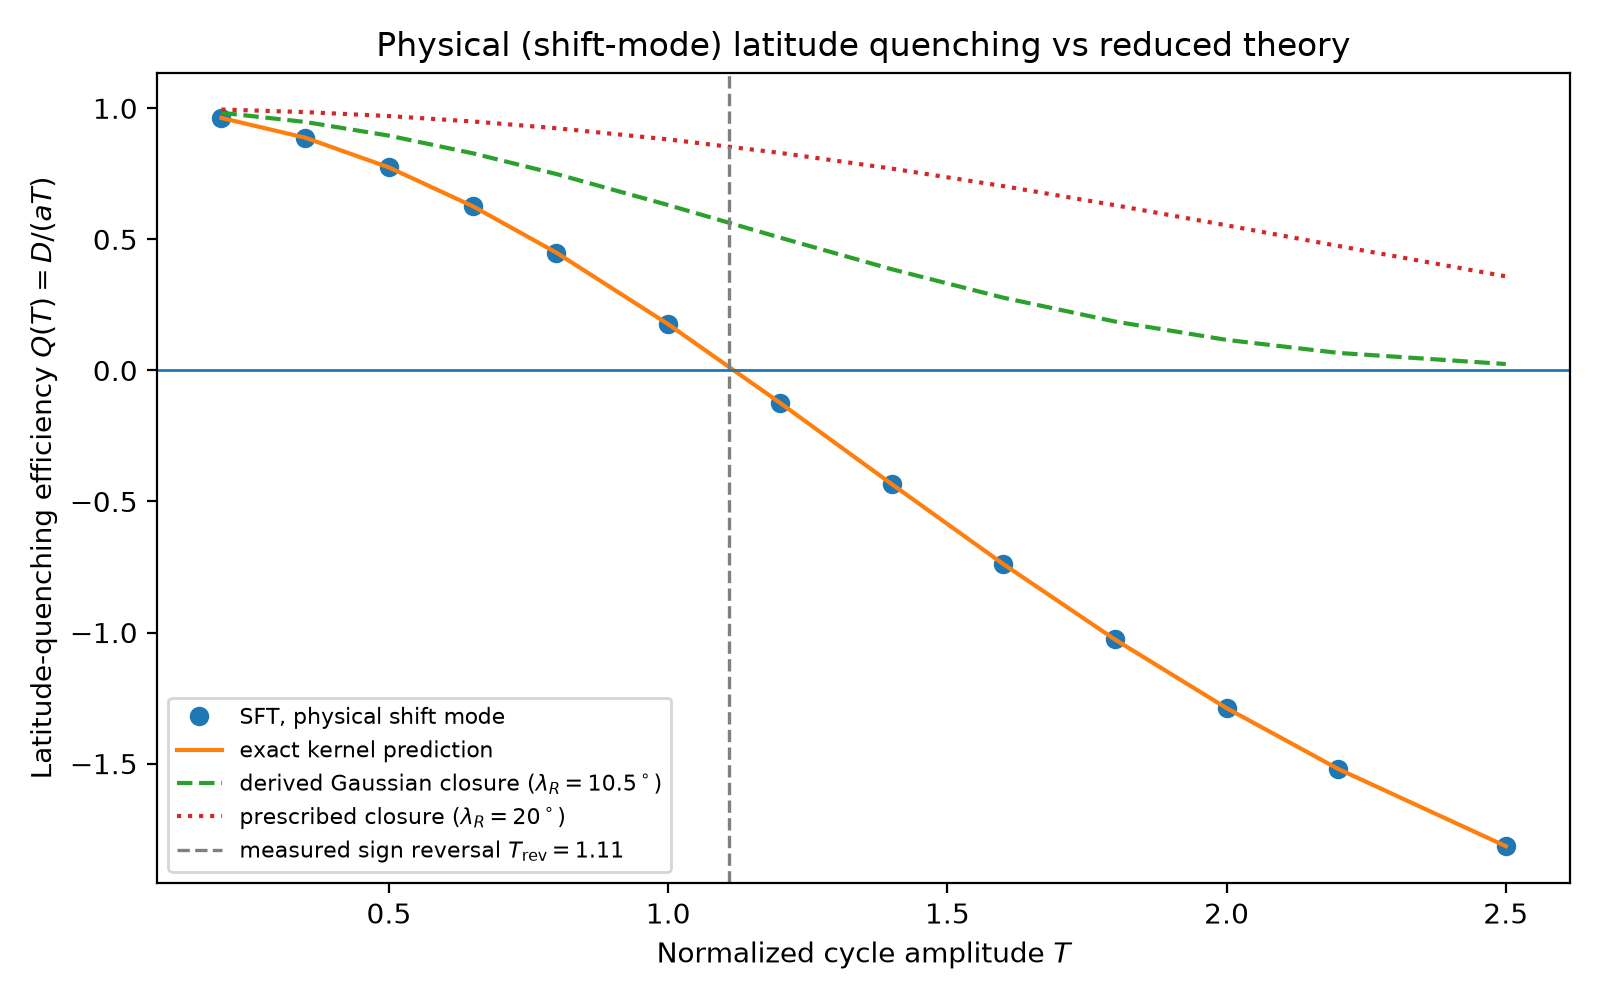
\includegraphics[width=\linewidth]{figV2_shift_validation.png}
\caption{Physical (shift-mode) latitude quenching in efficiency units
$Q(T)=D/(aT)$: the SFT scan, the exact kernel prediction, and the Gaussian
closures with the derived and prescribed effectivity ranges. The response
reverses sign at $T_{\rm rev}=1.11$, beyond the domain of any positive
closure.}
\label{fig:shift_validation}
\end{figure}

\subsection{Physical converging inflows}

Explicit converging inflows modify the transport operator, so no kernel
prediction exists -- the hardest test for a source-side factor. At the
reference inflow amplitude ($2~{\rm m~s^{-1}}$ at $T=1$, scaling as
$T^2$), the effective algebraic strength at the calibration point is
$b_{\rm eff}(T{=}1)=0.40$, with a leading-order fit $b_{\rm I}\simeq0.42$
over $T\le1.2$; the algebraic form is adequate for weak-to-moderate
cycles, but $b_{\rm eff}$ grows with $T$ (full-scan fit $1.5$): the
physical nonlinearity is super-quadratic, and the constant-$b$ Pad\'e form
under-predicts the suppression of strong cycles. At $5~{\rm m~s^{-1}}$ the
dipole reverses sign at $T=1.40$ -- over-quenching to reversal, again
outside the domain of positive closures. A useful cross-calibration
follows: the value $b_{\rm I}=0.2$ adopted from \citet{Talafha2025}
corresponds to inflow amplitudes of roughly $1~{\rm m~s^{-1}}$ at cycle
maximum in this model's convention.

\section{Multi-Cycle Coupling and the Memory-Corrected Map}
\label{sec:multicycle}

The reduced map~(\ref{eq:cycle_map}) assumes each cycle builds its dipole
from a clean slate. By linearity of the transport, the end-of-cycle dipole
in a sequence of coupled cycles obeys, exactly,
%
\begin{equation}
D_n
=
s_n\,a\,T_nQ(T_n)
+
w^{\rm T}G_P\,B_{n-1},
\label{eq:exact_recurrence}
\end{equation}
%
where $s_n$ is the source polarity of cycle $n$ (Hale alternation), the
first term is the new-flux contribution, $G_P$ the one-period propagator,
and $B_{n-1}$ the field at the end of the previous cycle. Collapsing the
memory term to a scalar, $w^{\rm T}G_PB_{n-1}\approx rD_{n-1}$, and
setting $T_n=k|D_{n-1}|$ with $D_0=ka$, gives on the successful-reversal
branch the \emph{memory-corrected map}
%
\begin{equation}
T_{n+1}
=
T_n\left[D_0Q(T_n)-r\right],
\label{eq:memory_map}
\end{equation}
%
with fixed point $D_0Q(T_*)=1+r$, existence threshold $D_0>1+r$, and
period doubling at $q(T_*)\ge2/(1+r)$.

For the reference transport with $\tau=\infty$ the memory parameter is
large: the remnant dipole survives one period with $r=0.986$, and its
asymptotic decay proceeds only through cross-equatorial diffusive
annihilation of the polar caps, exponentially slow in the magnetic
Reynolds number $R_{\rm m}=u_0R_\odot/\eta\approx17$. Almost half of the
dynamo gain is thus spent reversing the previous cycle's polar field --
the map-level manifestation of the flux-accumulation behaviour of
decay-free SFT models \citep{Schrijver2002,Baumann2006}.

Long multi-cycle SFT simulations with genuine feedback
($T_{n+1}=k|D_n|$, source polarity alternating), run with a matrix
stepper that reproduces the reference solver to $5\times10^{-14}$ and a
kernel-exact $Q(T)$ so that memory is the only difference between SFT and
map, confirm the corrected map quantitatively
(Figure~\ref{fig:bifurcation_comparison}): the one-step prediction error
falls from $97$~per~cent (memoryless) to $1.3$\,--\,$1.5$~per~cent; the
simulated attractor bifurcates to period two exactly at the corrected
analytic boundary $D_0=3.35$ (memoryless prediction: $2.80$) and follows
the corrected map through the subsequent cascade, including the phase of
the even--odd amplitude alternation and grand-minimum-like excursions in
the chaotic regime.

The reduced theory thus requires two transport constants, $(a,r)$, both
measurable from one linear run plus one source-free period. Because the
decay term commutes with the transport, $r(\tau)={\rm e}^{-P/\tau}
r(\infty)$ exactly (Section~\ref{sec:parameter_space}): observationally
calibrated decay times \citep[$\tau\sim5$\,--\,$10$~yr;][]{Schrijver2002,
Baumann2006} place the model in the weak-memory regime where the
memoryless map is a fair approximation, whereas decay-free models are in
the strong-memory regime where the correction is mandatory. The memory
term also makes consecutive cycles anticorrelated beyond what quenching
alone produces, connecting to the observed even--odd (Gnevyshev--Ohl)
alternation.

\begin{figure}
\centering
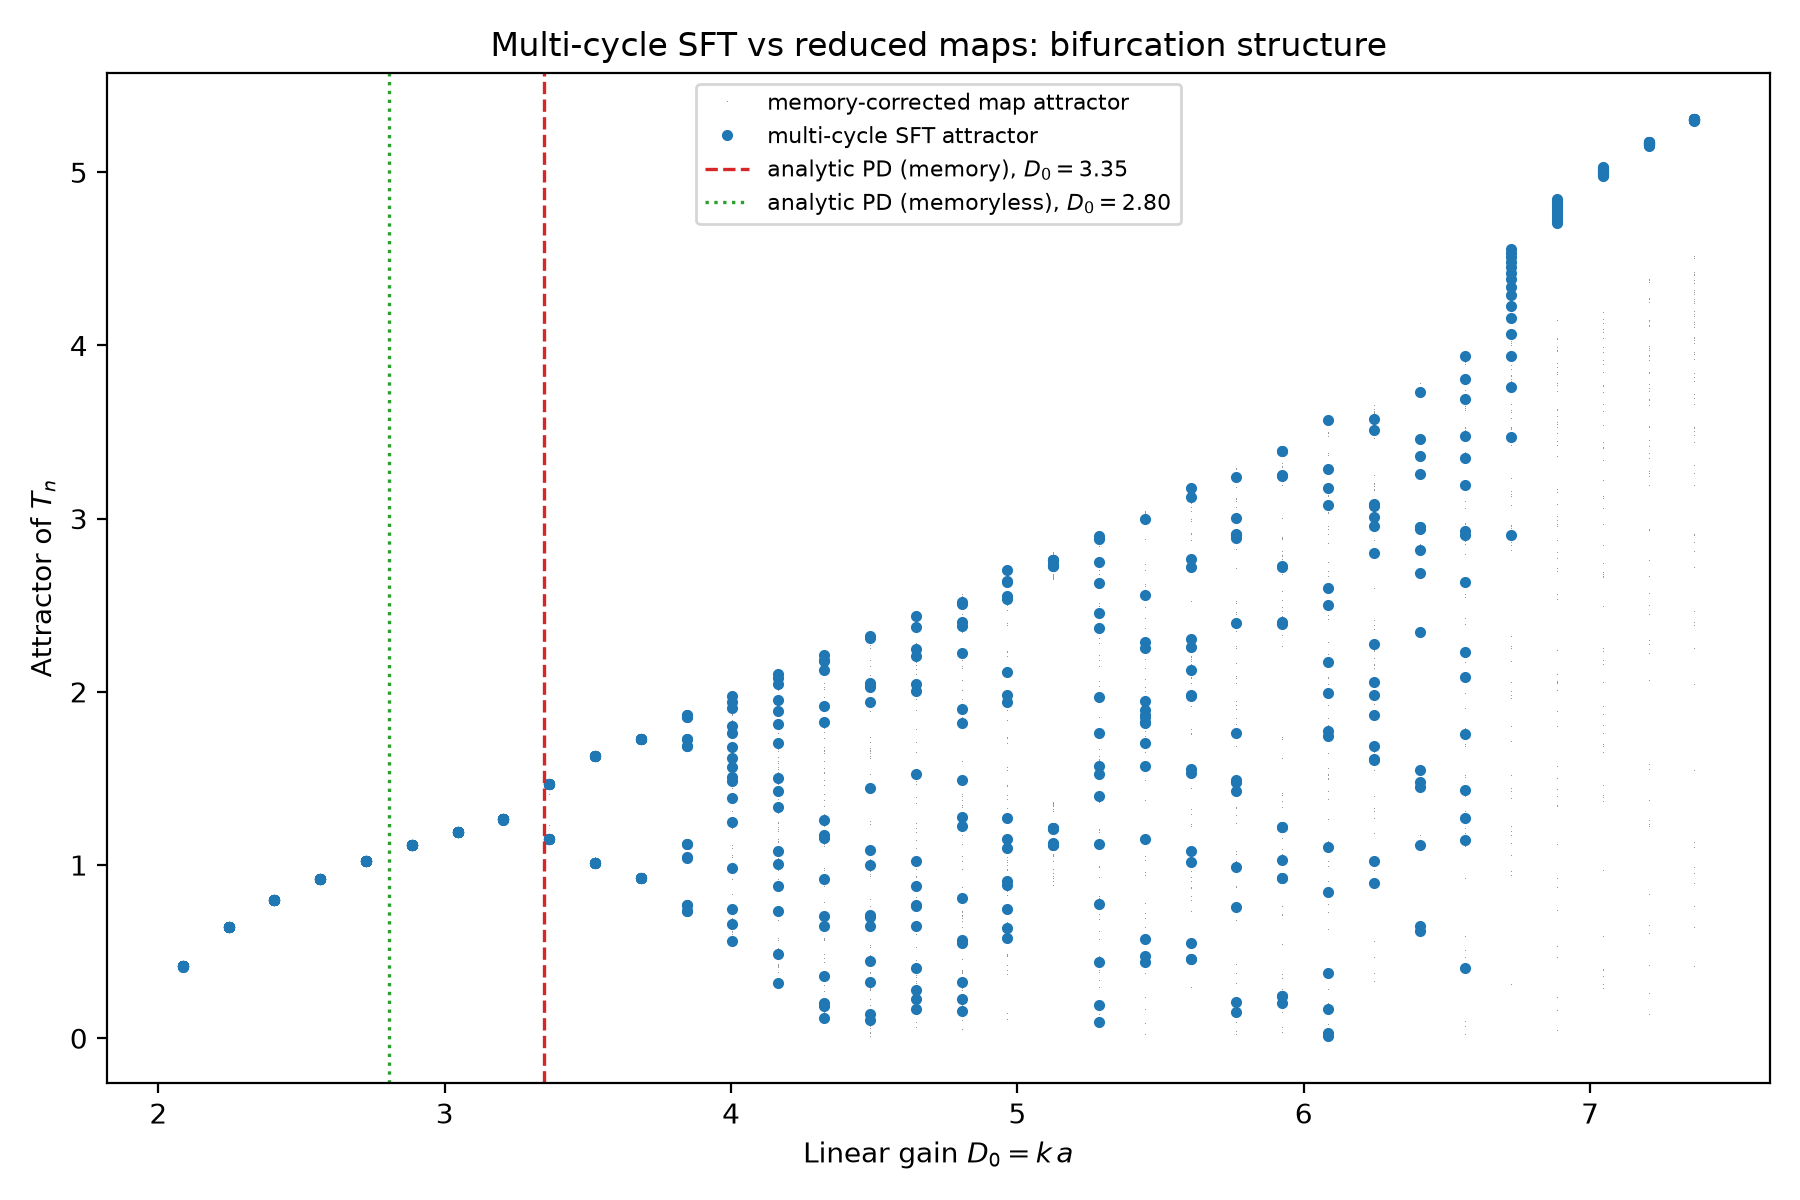
\includegraphics[width=\linewidth]{figM3_bifurcation_comparison.png}
\caption{Bifurcation structure of the multi-cycle SFT with dynamo
feedback compared with the memory-corrected map attractor. The vertical
lines mark the analytic period-doubling boundaries of the memoryless and
memory-corrected maps; the simulation follows the latter.}
\label{fig:bifurcation_comparison}
\end{figure}

\section{Transport Constants Across the Parameter Space}
\label{sec:parameter_space}

One adjoint solve per parameter set suffices to measure the derived
transport constants, so their behaviour can be mapped across the SFT
parameter space -- the reduced-theory counterpart of full parameter-space
optimisations \citep{PetrovayTalafha2019,Talafha2022}. Scanning
$\eta\in[100,1000]~{\rm km^2~s^{-1}}$ and $u_0\in[5,25]~{\rm m~s^{-1}}$
yields three regularities.

First, the pair-yield effectivity range collapses onto the quadrature
scaling law (Figure~\ref{fig:lambdaR_scaling})
%
\begin{equation}
\lambda_R^2
=
C^2\,\frac{\eta}{2u_0R_\odot}
+
w_0^2,
\qquad
C=1.008,
\quad
w_0=4.35^\circ,
\label{eq:quadrature_law}
\end{equation}
%
with a relative scatter of $2.5$~per~cent: the advection--diffusion
boundary-layer width with coefficient one, plus the finite source width
entering in quadrature. Over the scanned plane $\lambda_R$ runs from
$5.8^\circ$ to $22.7^\circ$, consistent with the values discussed by
\citet{PetrovayNagyYeates2020} and \citet{Talafha2022}.

Second, the sign-change latitude tracks the effectivity range,
%
\begin{equation}
\lambda_{\rm rev}
\approx
(2.33\pm0.25)\,\lambda_R ,
\label{eq:lambda_rev_law}
\end{equation}
%
so the domain of validity of positive latitude-quenching closures is
expressed directly in transport parameters: the emergence-weighted belt
must stay equatorward of about $2.3\lambda_R$.

Third, the decay time enters analytically. Because the decay term is
proportional to the identity, it commutes with the transport and factors
out of every kernel quantity exactly:
%
\begin{equation}
K(\tau)={\rm e}^{-(t_{\rm f}-t)/\tau}K(\infty),
\qquad
a(\tau)=\sum_k\omega_k\,{\rm e}^{-(t_{\rm f}-t_k)/\tau},
\qquad
r(\tau)={\rm e}^{-P/\tau}r(\infty),
\label{eq:tau_laws}
\end{equation}
%
while the shape of the yield function in latitude -- hence $\lambda_R$ and
$\lambda_{\rm rev}$ -- is invariant under $\tau$. These identities are
verified numerically at $\tau=5$~yr to within $10^{-4}$\,--\,$10^{-2}$. No
new scan is therefore needed for finite decay: the whole
$\tau$-dependence of the reduced theory is carried by two closed-form
factors applied to the $\tau=\infty$ constants.

In summary, any $(u_0,\eta,\tau)$ transport model of this family is
characterised, for the purposes of the reduced theory, by four numbers
measurable in about a second of computation: the linear yield $a$, the
effectivity range $\lambda_R$ (Equation~(\ref{eq:quadrature_law})), the
closure domain boundary $\lambda_{\rm rev}$
(Equation~(\ref{eq:lambda_rev_law})), and the cycle memory $r$
(Equation~(\ref{eq:tau_laws})).

\begin{figure}
\centering
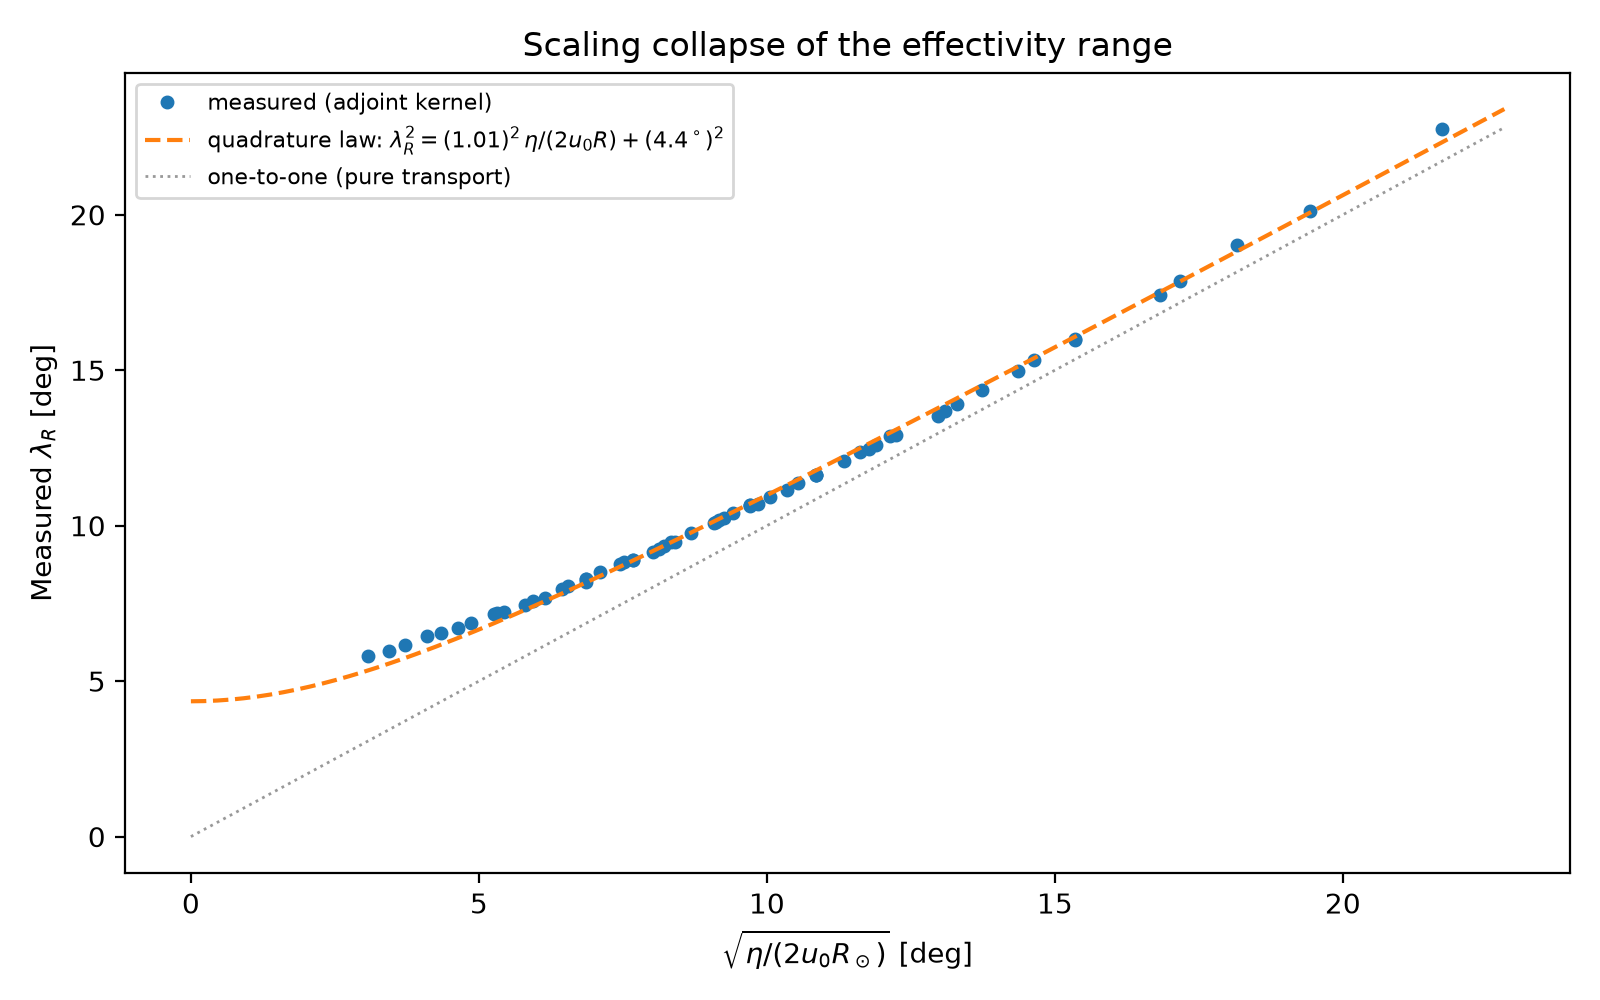
\includegraphics[width=\linewidth]{figP2_lambdaR_scaling.png}
\caption{Scaling collapse of the pair-yield effectivity range across the
$(\eta,u_0)$ plane onto the quadrature law of
Equation~(\ref{eq:quadrature_law}).}
\label{fig:lambdaR_scaling}
\end{figure}

\section{Summary and Conclusions}
\label{sec:conclusions}

\begin{enumerate}
\item
In controlled SFT experiments, the final signed axial dipole of a cycle
separates into the reduced form $P(T)=aTQ(T)$ to within a few per cent
over $T\in[0.2,2.5]$, with the latitude-quenching factor referenced
consistently to the drifting activity belt through a closed-form envelope
average.
\item
The adjoint (dipole-yield) kernel of the transport operator makes the
reduction exact for source-side nonlinearities: it defines $a$, verifies
the duality identity to $10^{-15}$, and organises the latitude closures
into a ladder whose error falls to $5\times10^{-5}$ with yield-weighted
time moments.
\item
The stability of the reduced cycle map is governed by the quenching
stiffness $q=-\rmd\ln Q/\rmd\ln T$: fixed points exist and are unique for
$D_0>1$; a single algebraic quenching can never period-double; Gaussian
latitude quenching always does for $D_0\ge{\rm e}$; and the measured
single-cycle response function determines the map multiplier exactly.
\item
Physically implemented nonlinearities respect sharp domain boundaries:
the ring-pair yield changes sign at $\lambda_{\rm rev}\approx2.3\lambda_R$,
so a genuine poleward belt displacement over-quenches the dipole to sign
reversal at $T\simeq1.1$ for the reference parameters, beyond the reach of
any positive multiplicative closure -- while the kernel predicts the full
signed response exactly. Physical inflows follow the algebraic closure to
$T\simeq1.2$ at observationally calibrated strengths.
\item
Without flux decay, the polar field survives almost entirely between
cycles ($r\simeq0.99$) and the memoryless cycle map fails structurally;
the memory-corrected map $T_{n+1}=T_n[D_0Q(T_n)-r]$ reproduces the
multi-cycle simulations quantitatively. The decay time sets the memory
regime analytically through $r(\tau)={\rm e}^{-P/\tau}r(\infty)$.
\item
Across the SFT parameter space the derived constants obey simple laws --
the quadrature scaling~(\ref{eq:quadrature_law}) for $\lambda_R$, the
proportionality~(\ref{eq:lambda_rev_law}) for the domain boundary, and
the closed-form $\tau$-dependence~(\ref{eq:tau_laws}) -- so that any
transport model of this family is summarised by four cheaply measurable
numbers $(a,\lambda_R,\lambda_{\rm rev},r)$.
\end{enumerate}

%\begin{acks}
% TODO: acknowledgements and funding.
%\end{acks}

%\begin{authorcontribution}
%\end{authorcontribution}

%\begin{fundinginformation}
%\end{fundinginformation}

%\begin{dataavailability}
%The code and data that reproduce all results are available in the
%repository accompanying this paper.
%\end{dataavailability}

%\begin{conflict}
%The authors declare no conflicts of interest.
%\end{conflict}

%%%%%%%%%%%%%%%%%%%%%%%%%%%%%%%%%%%%%%%%%%%%%%%%%%%%%%%%%%%%%%%%%%
\begin{thebibliography}{}

\bibitem[Babcock(1961)]{Babcock1961}
Babcock, H.W.: 1961, The topology of the Sun's magnetic field and the
22-year cycle. \apj\ {\bf 133}, 572.

\bibitem[Baumann, Schmitt, and Sch\"ussler(2006)]{Baumann2006}
Baumann, I., Schmitt, D., Sch\"ussler, M.: 2006, A necessary extension of
the surface flux transport model. \aap\ {\bf 446}, 307.

\bibitem[Cameron and Sch\"ussler(2012)]{CameronSchussler2012}
Cameron, R.H., Sch\"ussler, M.: 2012, Are the strengths of solar cycles
determined by converging flows towards the activity belts? \aap\
{\bf 548}, A57.

\bibitem[Charbonneau(2020)]{Charbonneau2020}
Charbonneau, P.: 2020, Dynamo models of the solar cycle. \lrsp\ {\bf 17},
4.

\bibitem[Dasi-Espuig et al.(2010)]{DasiEspuig2010}
Dasi-Espuig, M., Solanki, S.K., Krivova, N.A., Cameron, R.,
Pe\~nuela, T.: 2010, Sunspot group tilt angles and the strength of the
solar cycle. \aap\ {\bf 518}, A7.

\bibitem[Jiang(2020)]{Jiang2020}
Jiang, J.: 2020, Nonlinear mechanisms that regulate the solar cycle
amplitude. \apj\ {\bf 900}, 19.

\bibitem[Jiao, Jiang, and Wang(2021)]{Jiao2021}
Jiao, Q., Jiang, J., Wang, Z.-F.: 2021, Sunspot tilt angles revisited:
dependence on the solar cycle strength. \aap\ {\bf 653}, A27.

\bibitem[Leighton(1964)]{Leighton1964}
Leighton, R.B.: 1964, Transport of magnetic fields on the Sun. \apj\
{\bf 140}, 1547.

\bibitem[Mart\'in-Belda and Cameron(2017)]{MartinBelda2017}
Mart\'in-Belda, D., Cameron, R.H.: 2017, Inflows towards active regions
and the modulation of the solar cycle: a parameter study. \aap\
{\bf 597}, A21.

\bibitem[Petrovay(2020)]{Petrovay2020}
Petrovay, K.: 2020, Solar cycle prediction. \lrsp\ {\bf 17}, 2.

\bibitem[Petrovay and Talafha(2019)]{PetrovayTalafha2019}
Petrovay, K., Talafha, M.: 2019, Optimization of surface flux transport
models for the solar polar magnetic field. \aap\ {\bf 632}, A87.

\bibitem[Petrovay, Nagy, and Yeates(2020)]{PetrovayNagyYeates2020}
Petrovay, K., Nagy, M., Yeates, A.R.: 2020, Towards an algebraic method
of solar cycle prediction. I. Calculating the ultimate dipole
contributions of individual active regions. \jswsc\ {\bf 10}, 50.

\bibitem[Schrijver, De Rosa, and Title(2002)]{Schrijver2002}
Schrijver, C.J., De Rosa, M.L., Title, A.M.: 2002, What is missing from
our understanding of long-term solar and heliospheric activity? \apj\
{\bf 577}, 1006.

\bibitem[Talafha et al.(2022)]{Talafha2022}
Talafha, M., Nagy, M., Lemerle, A., Petrovay, K.: 2022, Role of
observable nonlinearities in solar cycle modulation. \aap\ {\bf 660},
A92.

\bibitem[Talafha, Petrovay, and Opitz(2025)]{Talafha2025}
Talafha, M.H., Petrovay, K., Opitz, A.: 2025, Effect of nonlinear surface
inflows into activity belts on solar cycle modulation. \solphys\
{\bf 300}, 57.

\end{thebibliography}

\end{document}
